

\typeout{}\typeout{If latex fails to find aiaa-tc, read the README file!}
%

\documentclass[]{aiaa-tc}% insert '[draft]' option to show overfull boxes

\usepackage{amssymb}
\usepackage{amsmath}
\usepackage{esint}
\usepackage{mathdesign}
\title{AOE-6145 FVM Code Implementation and Validation}

\author{
  Robert Masti%
}

\AIAApapernumber{YEAR-NUMBER}
\AIAAconference{Conference Name, Date, and Location}
\AIAAcopyright{\AIAAcopyrightD{YEAR}}

% Define commands to assure consistent treatment throughout document
\newcommand{\eqnref}[1]{(\ref{#1})}
\newcommand{\class}[1]{\texttt{#1}}
\newcommand{\package}[1]{\texttt{#1}}
\newcommand{\file}[1]{\texttt{#1}}
\newcommand{\BibTeX}{\textsc{Bib}\TeX}
\newcommand{\pderiv}[2]{\frac{\partial #1}{\partial #2}}
\newcommand*{\rttensor}[1]{\overline{\overline{#1}}}

\begin{document}

\maketitle

\begin{abstract}
A computational investigation was undertaken into the finite volume method in application to problems on two dimensional curvilinear mesh's. The numerical method consisted of second order MUSCL extrapolation, and numerical flux using Van Leer's, and Roe's, method. Method of manufactured solutions was used to verify the observed order of accuracy to the formal order of accuracy, and to determine iterative error estimates. A supersonic thirty degree inlet was investigated and a total pressure loss was found numerically to be $\Delta P_t=1.36e6\;Pa$. The flow around an airfoil was investigated using different angles of attack; macroscopic quantities such as lift and drag showed agreement with experimental results within $10\%$ difference.
\end{abstract}

\section*{Nomenclature}

\begin{tabbing}
XXX \= \kill% this line sets tab stop
 $\rttensor{T}$ \> flux tensor \\
 $\rho$ \> density \\
 $u$ \> x-velocity \\
 $v$ \> y-velocity \\
 $P$ \> pressure \\
 $h_t$ \> total specific enthalpy\\
 $e_t$ \> total specific energy\\
 $\vec{U}$ \> vector of conserved variables\\
 $\hat{U}$ \> bulk velocity normal to cell interface\\ 
  FVM \> Finite Volume Method \\
  MMS \> Method of Manufactured Solutions \\
  $A$ \> area \\
  $\Psi$ \> flux limiter \\
  $i,j$ \> cell index\\
  $c_d$ \> drag coefficient\\
  $c_l$ \> lift coefficient\\
  $c$ \> chord length
\end{tabbing}

\section{Theory}

Euler equations in 2D Cartesian coordinates were solved using the finite volume method to reach steady state solutions for various problems. Method of Manufactured Solutions was used to validate the numerical method, and to determine an observed order of accuracy. The numerical method is able to solve structured curvilinear geometry, with Roe, and Van Leer, numerical flux. The Euler equations in strong conservative form assuming a calorically perfect gas can be written as
\begin{equation}\label{eq:eulrho}
  \pderiv{\rho}{t} + \nabla\cdot(\rho \vec{v}) = 0
\end{equation}
\begin{equation}\label{eq:eulmtm}
  \pderiv{\rho \vec{v}}{t} + \nabla\cdot(\rho \vec{v}\vec{v} + \mathbb{I} P) = 0
\end{equation}
\begin{equation}\label{eq:eulenergy}
  \pderiv{\rho e_t}{t} + \nabla\cdot(\rho h_t \vec{v}) = 0
\end{equation}
where $\rho$ is the density, $\vec{v}$ is the vector bulk velocity, $t$ is time, $\mathbb{I}$ is the identity matrix, $P$ is the pressure, $e_t$ is the total specific energy, and $h_t$ is the total specific enthalpy. This can be reduced to 
\begin{equation}\label{eq:eultensor}
  \pderiv{\vec{U}}{t} + \nabla\cdot\rttensor{T} = 0
\end{equation}
where $\vec{U}$ is the vector of conserved variables, and $\rttensor{T}$ is the flux tensor. Equation~\ref{eq:eultensor} is valid for all coordinate systems, but in 2D Cartesian coordinates it can be expanded to
\[
  \pderiv{}{t}
  \begin{bmatrix}
    \rho \\
    \rho u \\
    \rho v \\
    \rho e_t
  \end{bmatrix}
  + \pderiv{}{x}
  \begin{bmatrix}
    \rho u \\
    \rho u^2 + P \\
    \rho u v \\
    \rho u h_t
  \end{bmatrix}
  + \pderiv{}{x}
  \begin{bmatrix}
    \rho v \\
    \rho v u \\
    \rho v^2 + P \\
    \rho v h_t
  \end{bmatrix}
  =0
\]
where the first term is the conserved variable vector $\vec{U}$, the second term is the $\hat{x}$ direction flux, and the third term is the $\hat{y}$ direction flux. For a calorically perfect gas the total specific enthalpy can be related to the total specific energy by
\begin{equation} \label{eq:idealgas}
  h_t = e_t + \frac{P}{\rho}
\end{equation}

. Thus equations~\ref{eq:eulrho}-~\ref{eq:idealgas} combined make the closed system of governing equations used in this numerical model. There are modifications needed for curvilinear meshes on the fluxes see section~\ref{sec:nummod} for details.

FVM requires the equations in the weak form, so equations~\ref{eq:eulrho}-~\ref{eq:eulenergy} are integrated over the volume of a given cell, and with further simplification using the divergence theorem equation~\ref{eq:eultensor} reduces to
\begin{equation}\label{eq:eulfvm}
  \iiint\limits_V \pderiv{\vec{U}}{t} dV + \oiint \rttensor{T} \cdot \vec{dA} = 0
\end{equation}
where $V$ is the volume, and $A$ is the area. This equation is then discretized and solved using FVM. 

\section{Numerical Model}\label{sec:nummod}
Using cell integrated averaged quantities the basic 2D discretization of equation \ref{eq:eulfvm} can be written as
\begin{equation} \label{eq:euldisc}
  \pderiv{\vec{U}}{t}V_{i,j} + \sum_{k=1}^4\rttensor{T_k}\cdot \vec{A_k} = 0
\end{equation}
where ${i,j}$ is the location of a cell in the computational domain, and in 2D it will have 4 faces.  With the curvilinear meshes the fluxes and areas are converted to the computational domain ($i,j$) through normal vector components ($n_{\hat{x}}$ and $n_{\hat{y}}$) transformations. As an example the transformation of the $\hat{x}$ direction flux will become
\[
  \vec{F_{normal}} =
  \begin{bmatrix}
    \rho \hat{U} \\
    \rho u\hat{U} + P \\
    \rho \hat{U} v \\
    \rho \hat{U} h_t
  \end{bmatrix}
\]
where $\hat{U}$ is the projected bulk velocity normal to the cell surface. Similarly this can be done to obtain the $j$ direction flux. The fluxes in equation~\ref{eq:euldisc} must be evaluated at the interfaces of a given cell ${i,j}$, and this is done through reconstruction of the cell averaged solutions onto the interface. 


\subsection{MUSCL Extrapolation}\label{sec:nummod:MUSCL}
MUSCL (Monotone Upstream-centered Schemes for Conservation Laws) extrapolation is used to get a second order accurate numerical scheme. Extrapolation is needed to get the value of the conserved variables at the interface, and a first order method only uses the cells on either side of the interface. MUSCL uses three cells for the left state, and three cells for the right state, with one cell counted twice making it a five point stencil. Since MUSCL is an upwinding schemes it is prone to issues with stability in regions of high gradients such as shocks. To resolve this flux limiters are used that satisfy total variation diminishing (TVD), and monotonicity.

MUSCL extrapolation by itself in the $i$ direction can be written as
\begin{equation}\label{eqn:MUSCLleft}
  U_{i+1/2, j}^L = U_{i,j} + \frac{1}{2}\left(U_{i,j} - U_{i-1, j}\right)
\end{equation}
\begin{equation}\label{eqn:MUSCLright}
  U_{i+1/2, j}^R = U_{i+1, j} - \frac{1}{2}\left(U_{i+2, j} - U_{i+1, j}\right)
\end{equation}
where the whole integer $i$ or $j$ represent cells, and the half integer $i+1/2$ represents the interface on the right ($+\hat{x}$). This approach can be similarly done for the left, top, and bottom interfaces of the cell.

\subsubsection{Flux Limiters}\label{sec:nummod:fluxlimit}
In order to fix MUSCL's shock capturing issues a limiter can be used to reduce the numerical scheme to first order in regions of large gradients. A limiter if applied must ensure TVD, and monotonicity. TVD is the condition that the scalar conservation law in equation~\ref{eqn:mhdvecflux} integrated over the domain does not increase with time. Monotonicity is ensuring that the reconstructed interface value does not result in a new extrema from extrapolation. Reducing the MUSCL scheme to first order accuracy in regions of sharp gradients must be done so in a way that the regions of smooth gradients are still second order accurate.

Using the ratio of consecutive variation of the conserved variables evaluated at the interface can be used to detect large gradients. An additional term $\Psi(r)$ is added to the second part of equations~\ref{eqn:MUSCLleft}, and~\ref{eqn:MUSCLright}, where r is the ratio of consecutive variations. Their are conditions on $\Psi$ that must be followed to ensure TVD, and monotonicity, which can be followed on the Sweby diagram.\cite{leveque2002}. Thus flux limiters with equations~\ref{eqn:MUSCLleft}-\ref{eqn:MUSCLright} the second order accurate upwinding interface reconstruction on conserved variables is defined. This approach is fully upwinded, but a $\kappa$ scheme can be introduced to get partially upwinding reconstruction instead. The $\kappa$ scheme can be written as

\begin{equation}\label{eqn:MUSCLleft}
  U_{i+1/2, j}^L = U_{i,j} +\frac{epsilon}{4}\left((1-\kappa)\Psi_{i+1/2,j}^+(U_{i,j} - U_{i-1, j})+ (1+\kappa)\Psi_{i+1/2,j}^-(U_{i+1,j} - U_{i, j})\right)
\end{equation}
\begin{equation}\label{eqn:MUSCLright}
  U_{i+1/2, j}^R = U_{i+1, j} - \frac{epsilon}{4}\left((1-\kappa)\Psi_{i+3/2,j}^-(U_{i+2,j} - U_{i+1, j})+ (1+\kappa)\Psi_{i+1/2,j}^+(U_{i+1,j} - U_{i, j})\right)
\end{equation}
where the $\Psi^{\pm}$ determines whether to use the ratio consecutive variation in the forward ($+i$)or reverse ($-i$) direction. $\kappa$ is used to limit the amount of upwinding used in the extrapolation, and $\epsilon$ is used to provide explicit control over the change from 1st to 2nd order extrapolation.

\subsection{Numerical Flux}
The conserved variable reconstructed onto the interfaces need to be used to compute numerical flux. One of the numerical fluxes used in this scheme is the Van Leer flux vector splitting (FVS). FVS separates the flux into a convective, and a pressure flux that is found through conditionally modifying the left an right mach numbers based on the direction of speed. This scheme is chosen due to the properties of flux consistency, continuity, and continuous differentiability. 

The other flux used in this scheme is a flux difference splitting scheme (FDS). One of the least diffusive FDS flux schemes is the Roe's FDS scheme. Roe's scheme uses all of the eigenvalues and eigenvectors of the flux jacobian to evaluate the numerical flux with the differential vector of characteristic variables. The eigenvalue and eigenvector components are evaluated using a square root of density average of the left and right state primitive variables which are defined as the Roe averaged variables.

\section{Results}
Three cases were studied using this numerical scheme. The first is to perform a code verification study using MMS by examining the supersonic and subsonic cases described in Roy et. al. 2004.\cite{Roy2004} The second case study is the supersonic flow through a simplified 2D 30$^o$ inlet. The third case study is the flow around an NACA64A airfoil with a thickness to chord ratio of $6$\% using different angles of attack. 

\subsection{Case 1: Method of Manufactured Solutions}
Using the solution and the source terms from Roy et. al. 2004 the observed order of accuracy is found using MMS.\cite{Roy2004} MMS was conducted on systematically refined meshes (nodes) of size 9x9, 17x17, 33x33, 65x65, 129x129, and 257x257. The boundary conditions are set as the exact solution determined from the manufactured solution, and the source terms are created by an analytical expression determined by evaluating~\ref{eq:eultensor} with the exact solution. 

Figure~\ref{fig:OASS} shows the observed order for the supersonic manufactured solution, and as the grid is refined (lower $h$) the observed order approach 2 which matches the formal order. Similarly figure~\ref{fig:OASB} shows the observed order for the subsonic manufactured solution, and it also shows close agreement with the formal order of 2. In figure~\ref{fig:IESS} the supersonic and subsonic iterative error and residual are shown for the 65x65 grid. The iterative error is on the order of 0.1\% for the medium sized mesh, and varies for the different primitive variables. It asymptotically approaches a value that will change dependent on the resolution of the numerical solution with respect to the manufactured solution. This shows that the iterations needed to reach near the asymptotic error are 600, and 1500, for the supersonic solution, and subsonic solution, respectively. Also any iterative residual smaller than $\approx1e-4$ is sufficient in reaching the best solution with respect to the iterative error. The local discretization error is shown in figure~\ref{fig:DESS} and the characteristic transport lines are visible. In addition the solutions for the subsonic and supersonic manufactured solution are shown in figure~\ref{fig:SS} which can be directly compared to Roy et. al. 2004 figure 1, and figure 6.\cite{Roy2004}

\begin{figure}[!htb]
  \minipage{0.49\textwidth}
  \label{fig:OASS}
  \centering
  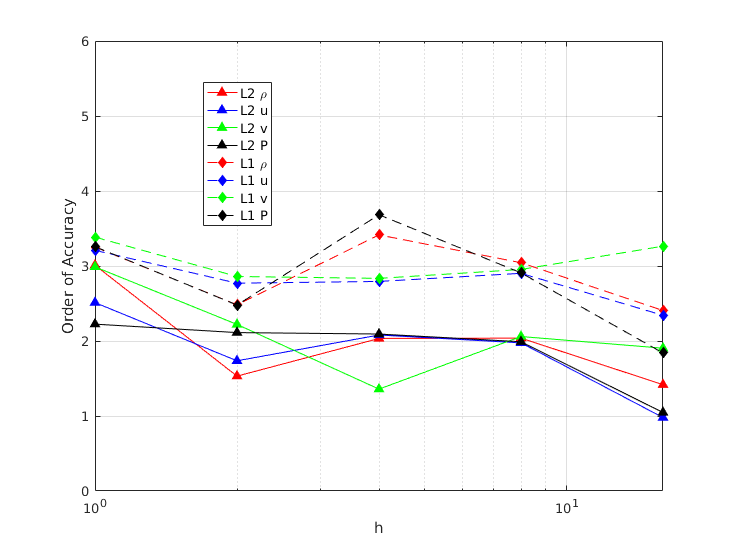
\includegraphics[width=\linewidth]{figures/OA_SS}
  \caption{Observed order of accuracy using 2nd order Van Leer FVS for the supersonic manufactured solution.}
  \endminipage\hfill
  \minipage{0.49\textwidth}
  \label{fig:OASB}
  \centering
  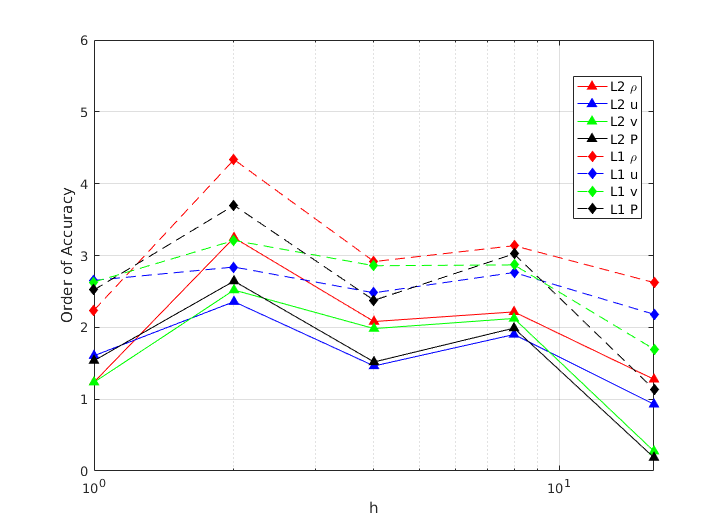
\includegraphics[width=\linewidth]{figures/OA_SB}
  \caption{Observed order of accuracy using 2nd order Van Leer FVS for the subsonic manufactured solution.}
  \endminipage\hfill
\end{figure}

\begin{figure}[!htb]
  \minipage{0.49\textwidth}
  \centering
  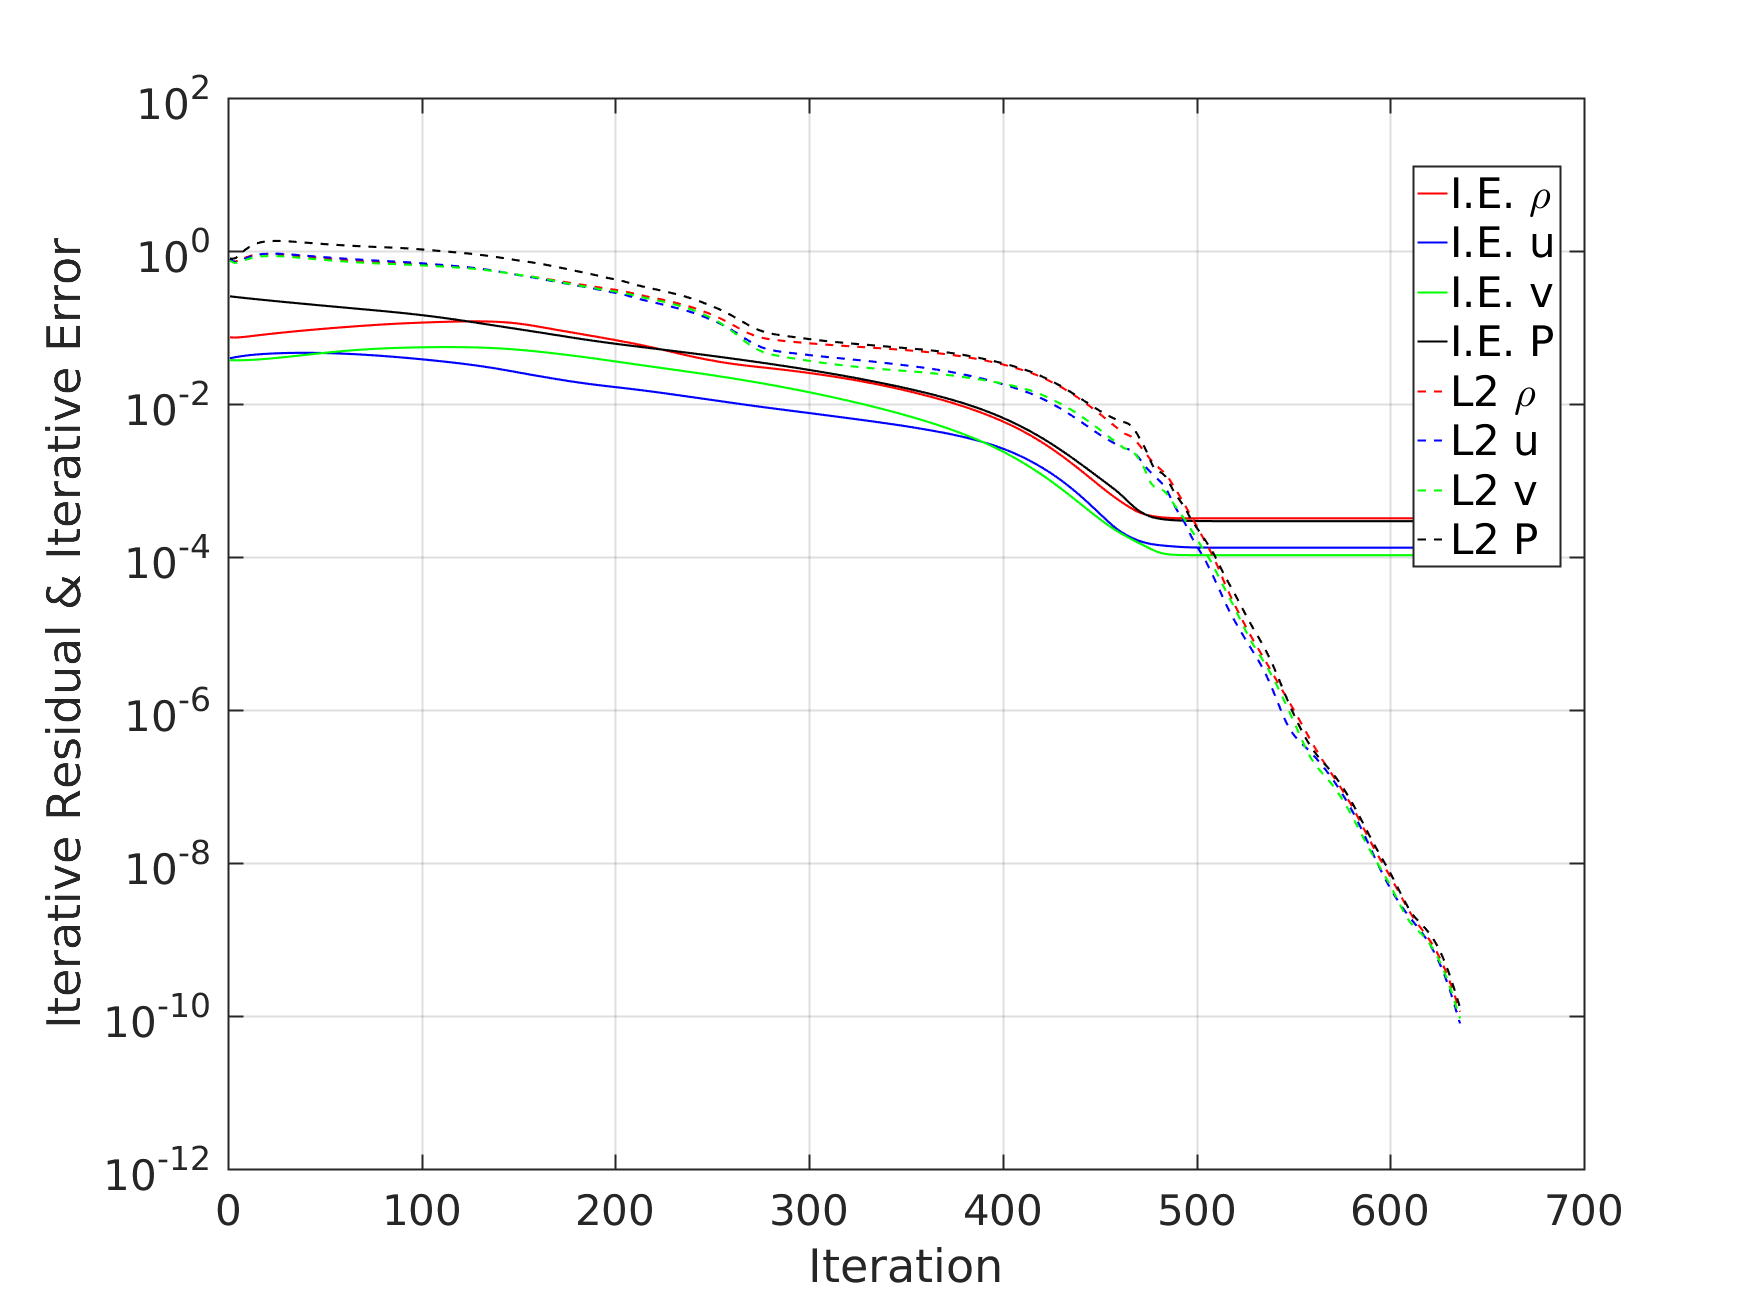
\includegraphics[width=\linewidth]{figures/Iter_SS}
  \caption{Iterative error (I.E.), and Iterative residual using 2nd order Van Leer FVS for the supersonic manufactured solution on the 65x65 mesh.}
  \label{fig:IESS}
  \endminipage\hfill
  \minipage{0.49\textwidth}
  \centering
  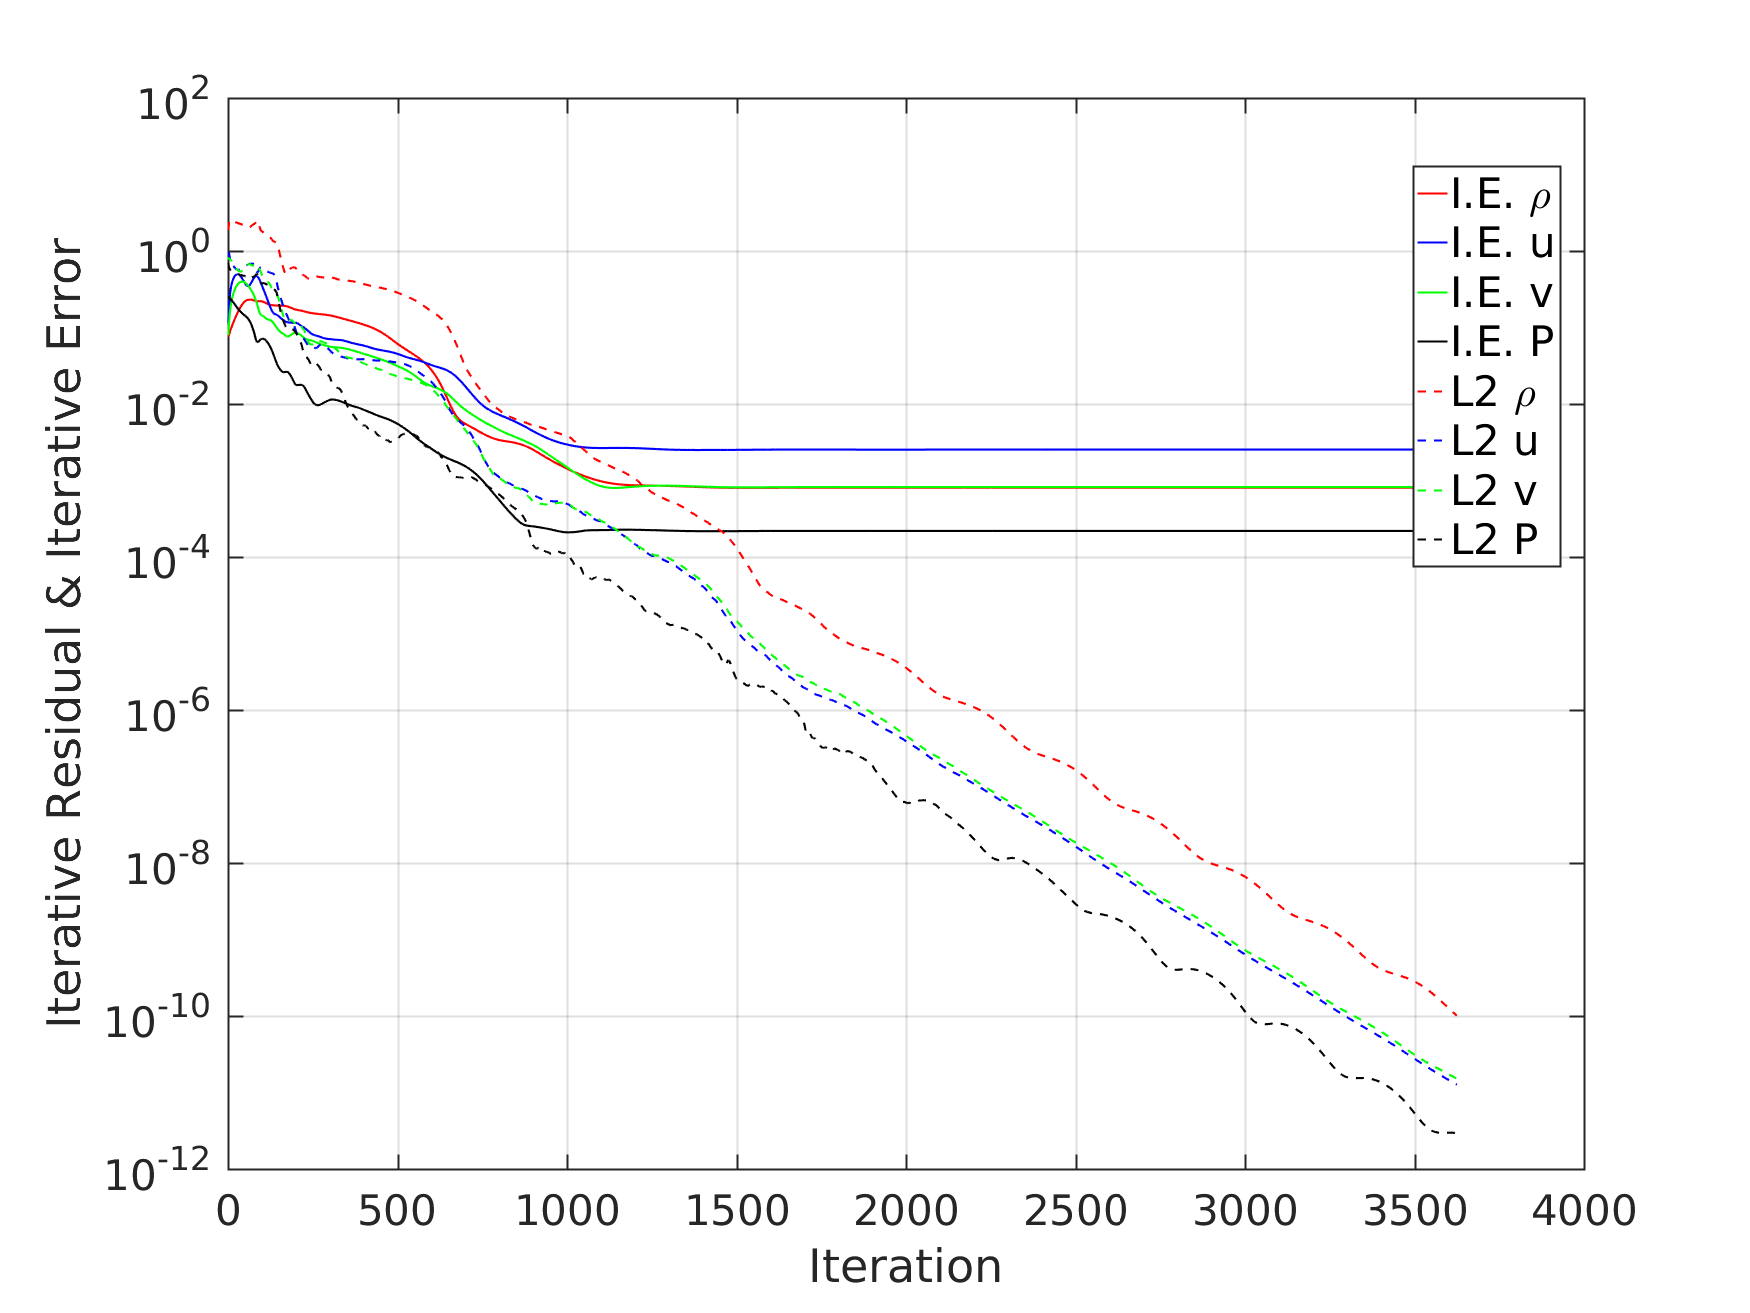
\includegraphics[width=\linewidth]{figures/Iter_SB}
  \caption{Iterative error (I.E.), and Iterative residual using 2nd order Van Leer FVS for the subsonic manufactured solution on the 65x65 mesh.}
\label{fig:IESB}
  \endminipage\hfill
\end{figure}

\begin{figure}[!htb]
  \minipage{0.49\textwidth}
  \centering
  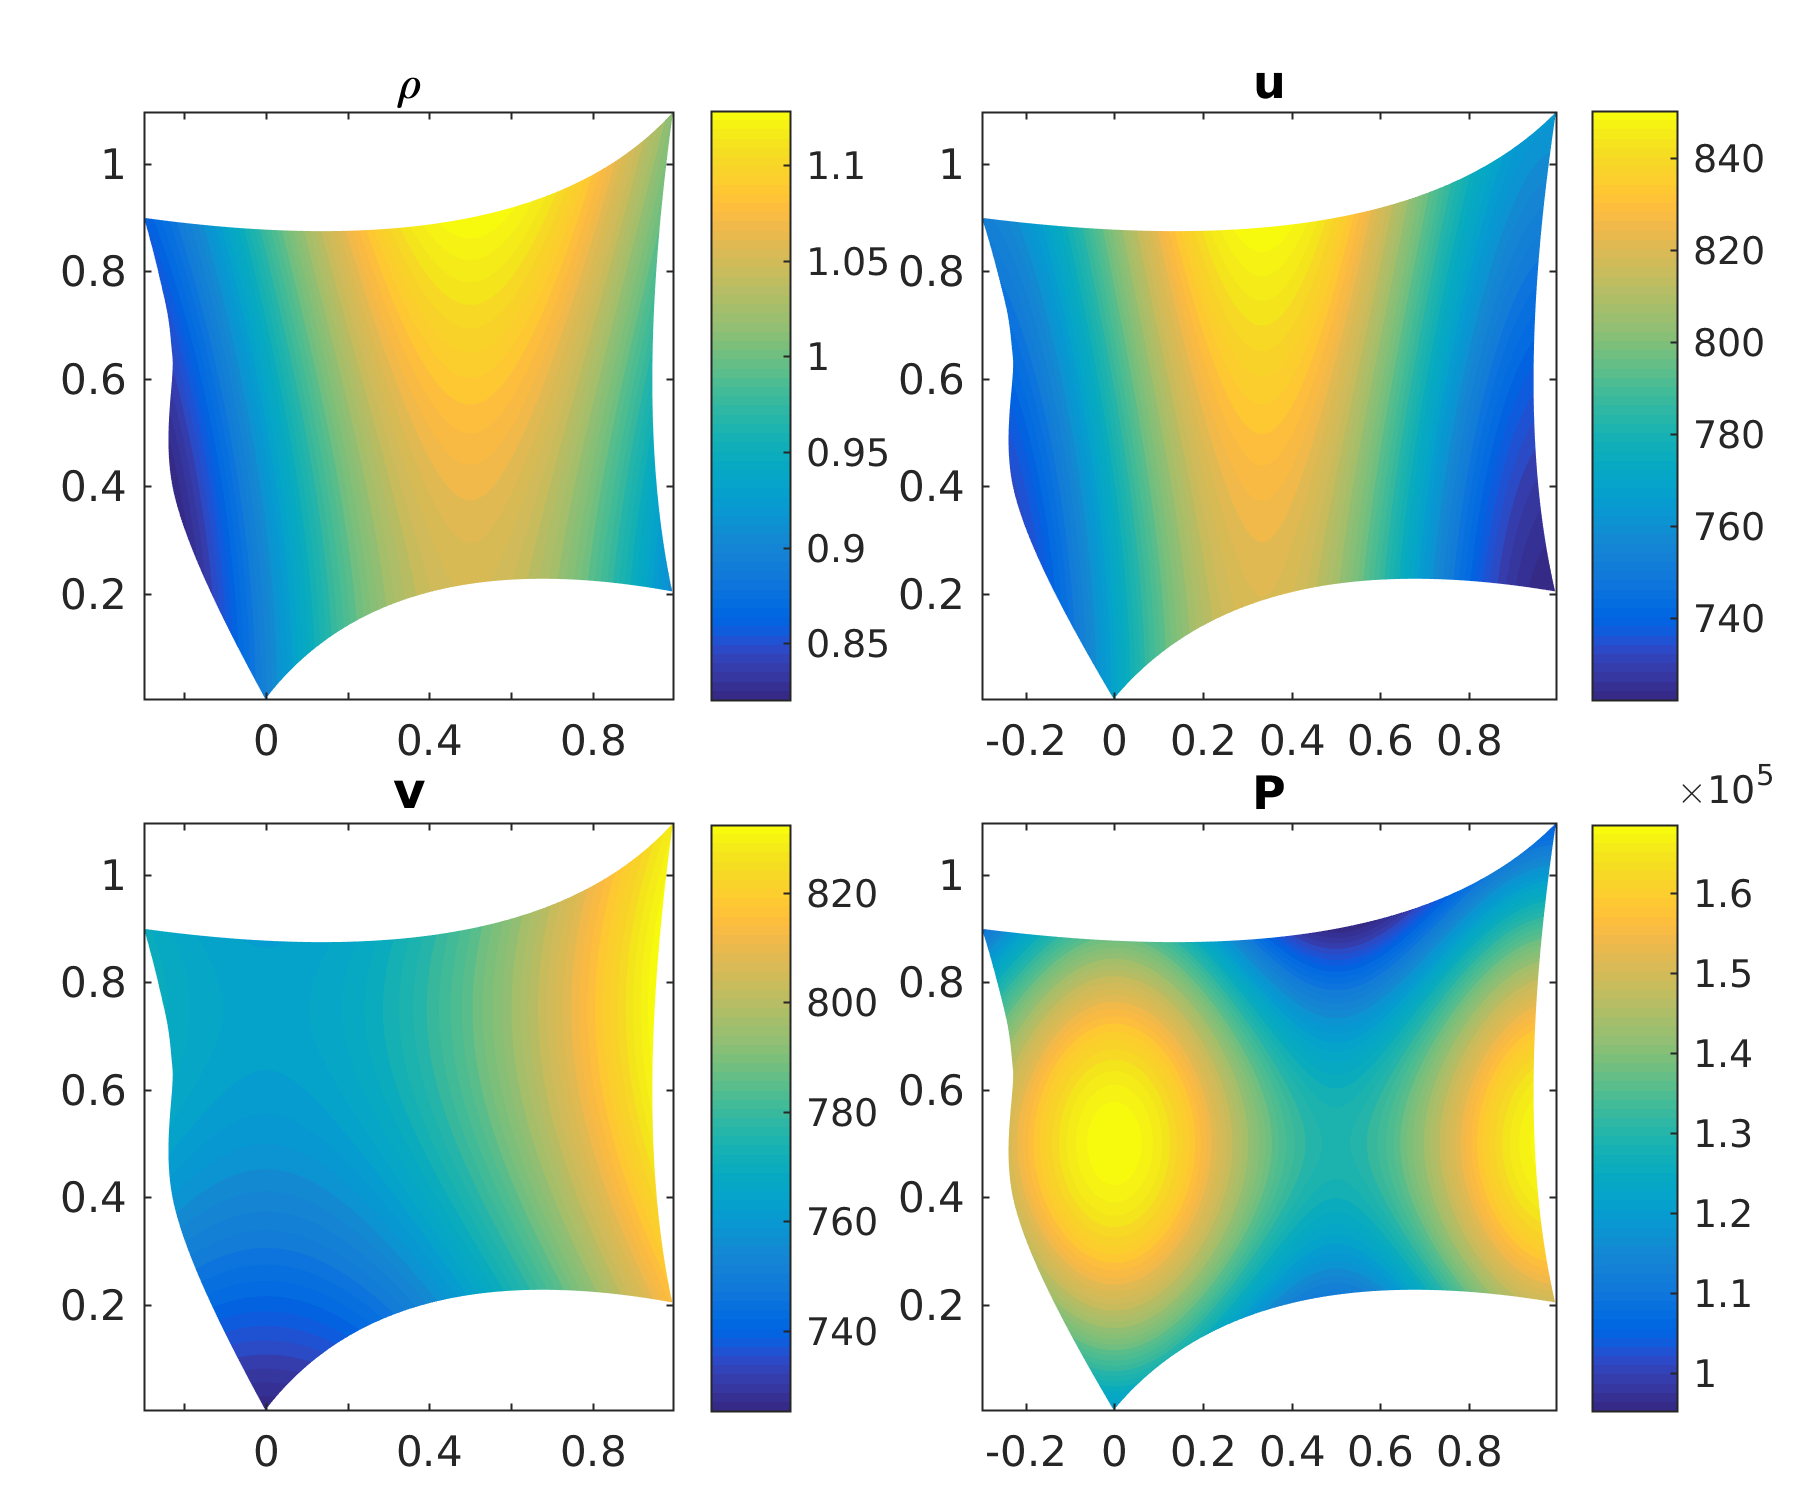
\includegraphics[width=\linewidth]{figures/MMS_mesh6_SS_soln}
  \caption{Numerical solution using 2nd order Van Leer FVS for the supersonic manufactured solution on the 257x257 mesh.}
  \label{fig:SS}
  \endminipage\hfill
  \minipage{0.49\textwidth}
  \centering
  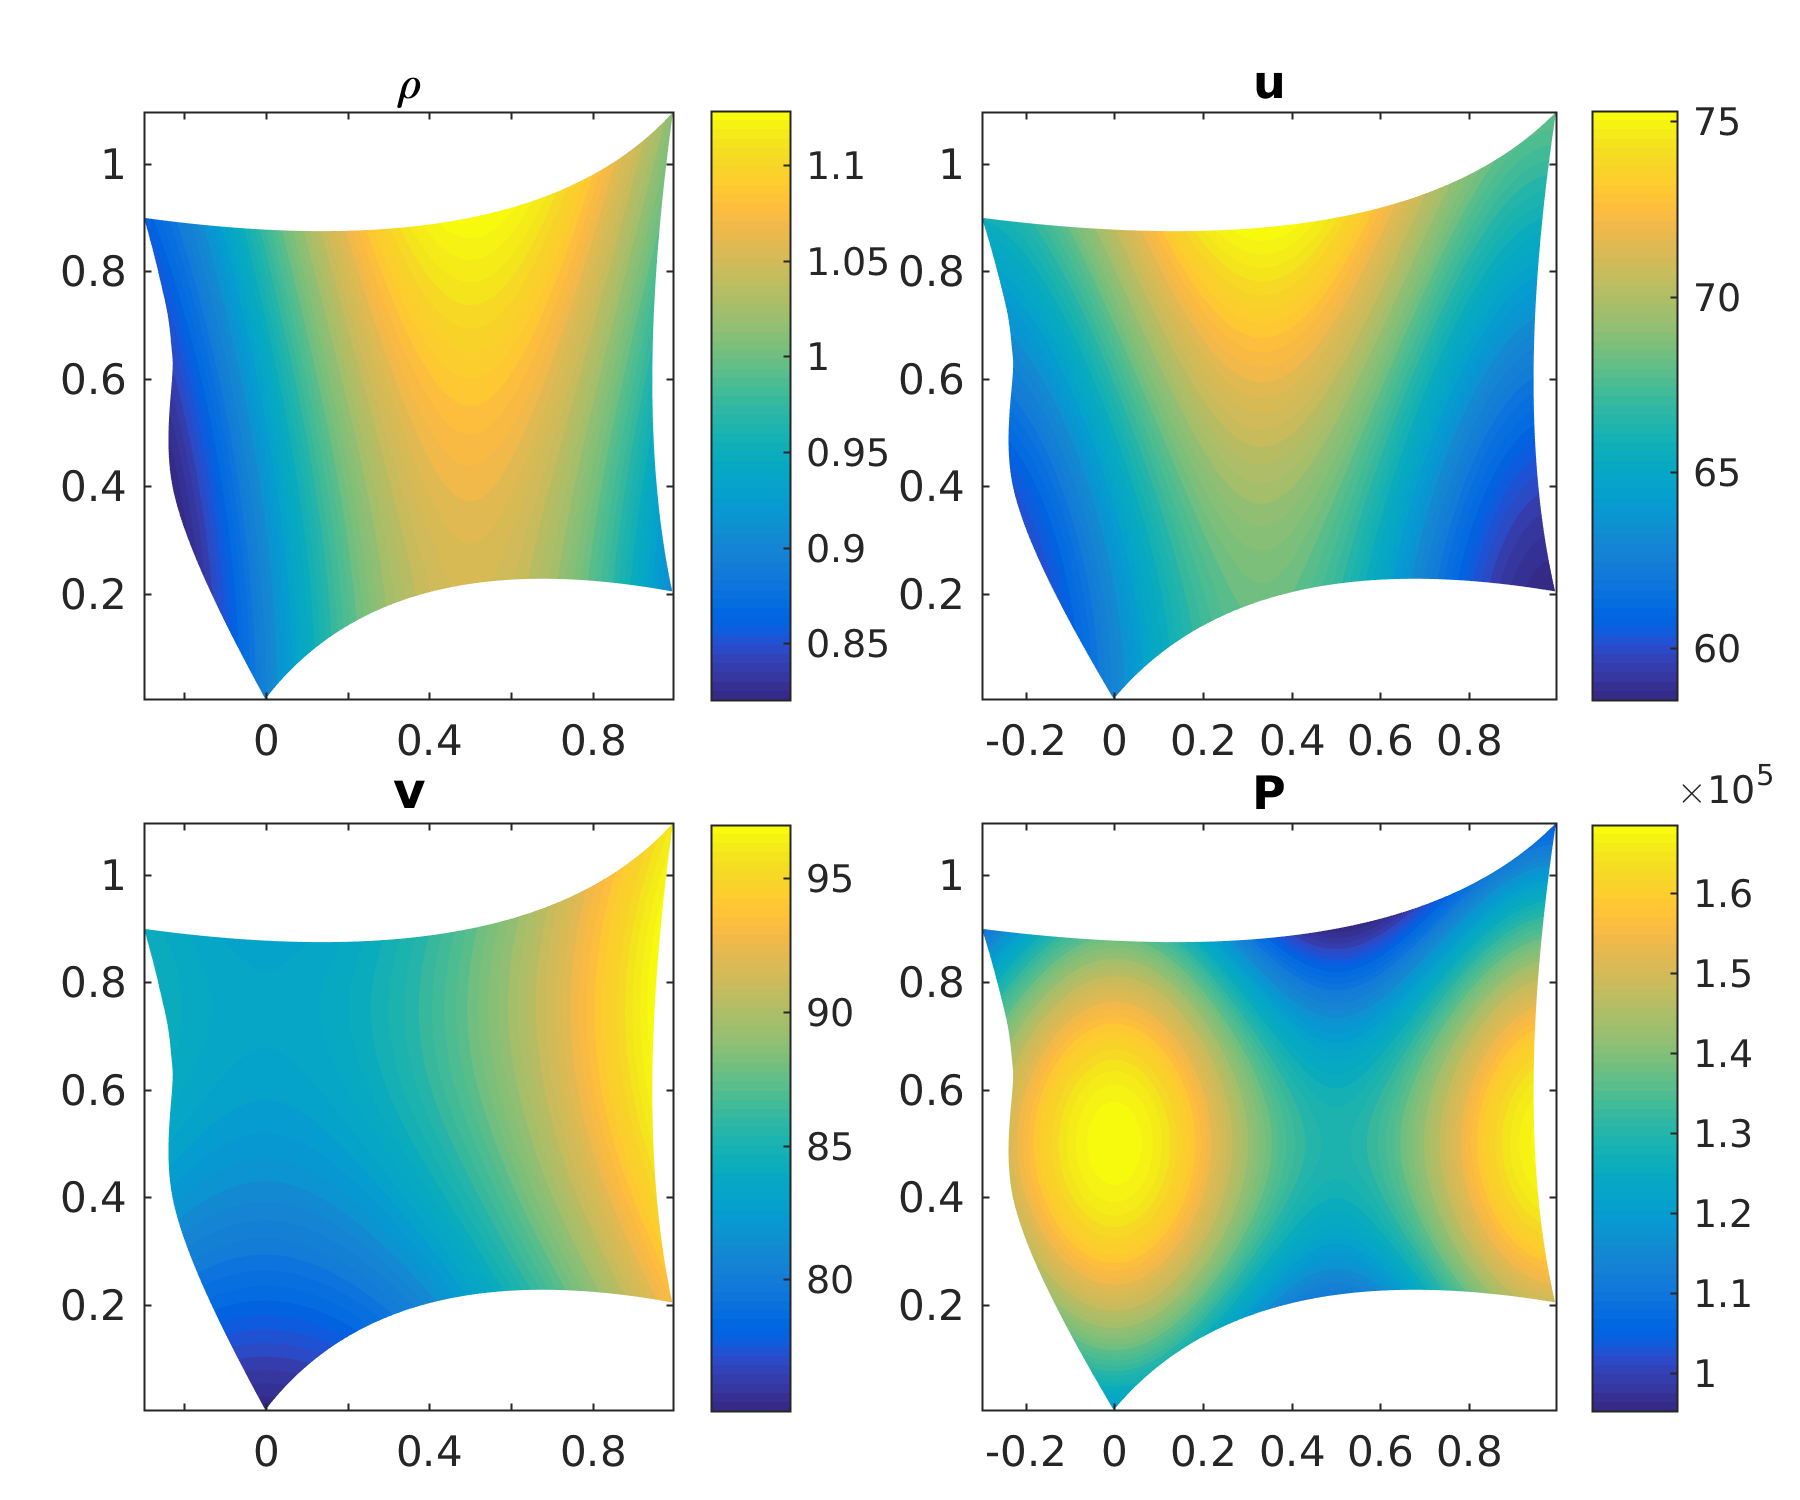
\includegraphics[width=\linewidth]{figures/MMS_mesh6_SB_soln}
  \caption{Numerical solution using 2nd order Van Leer FVS for the subsonic manufactured solution on the 257x257 mesh.}
\label{fig:SB}
  \endminipage\hfill
\end{figure}

\begin{figure}[!htb]
  \minipage{0.49\textwidth}
  \centering
  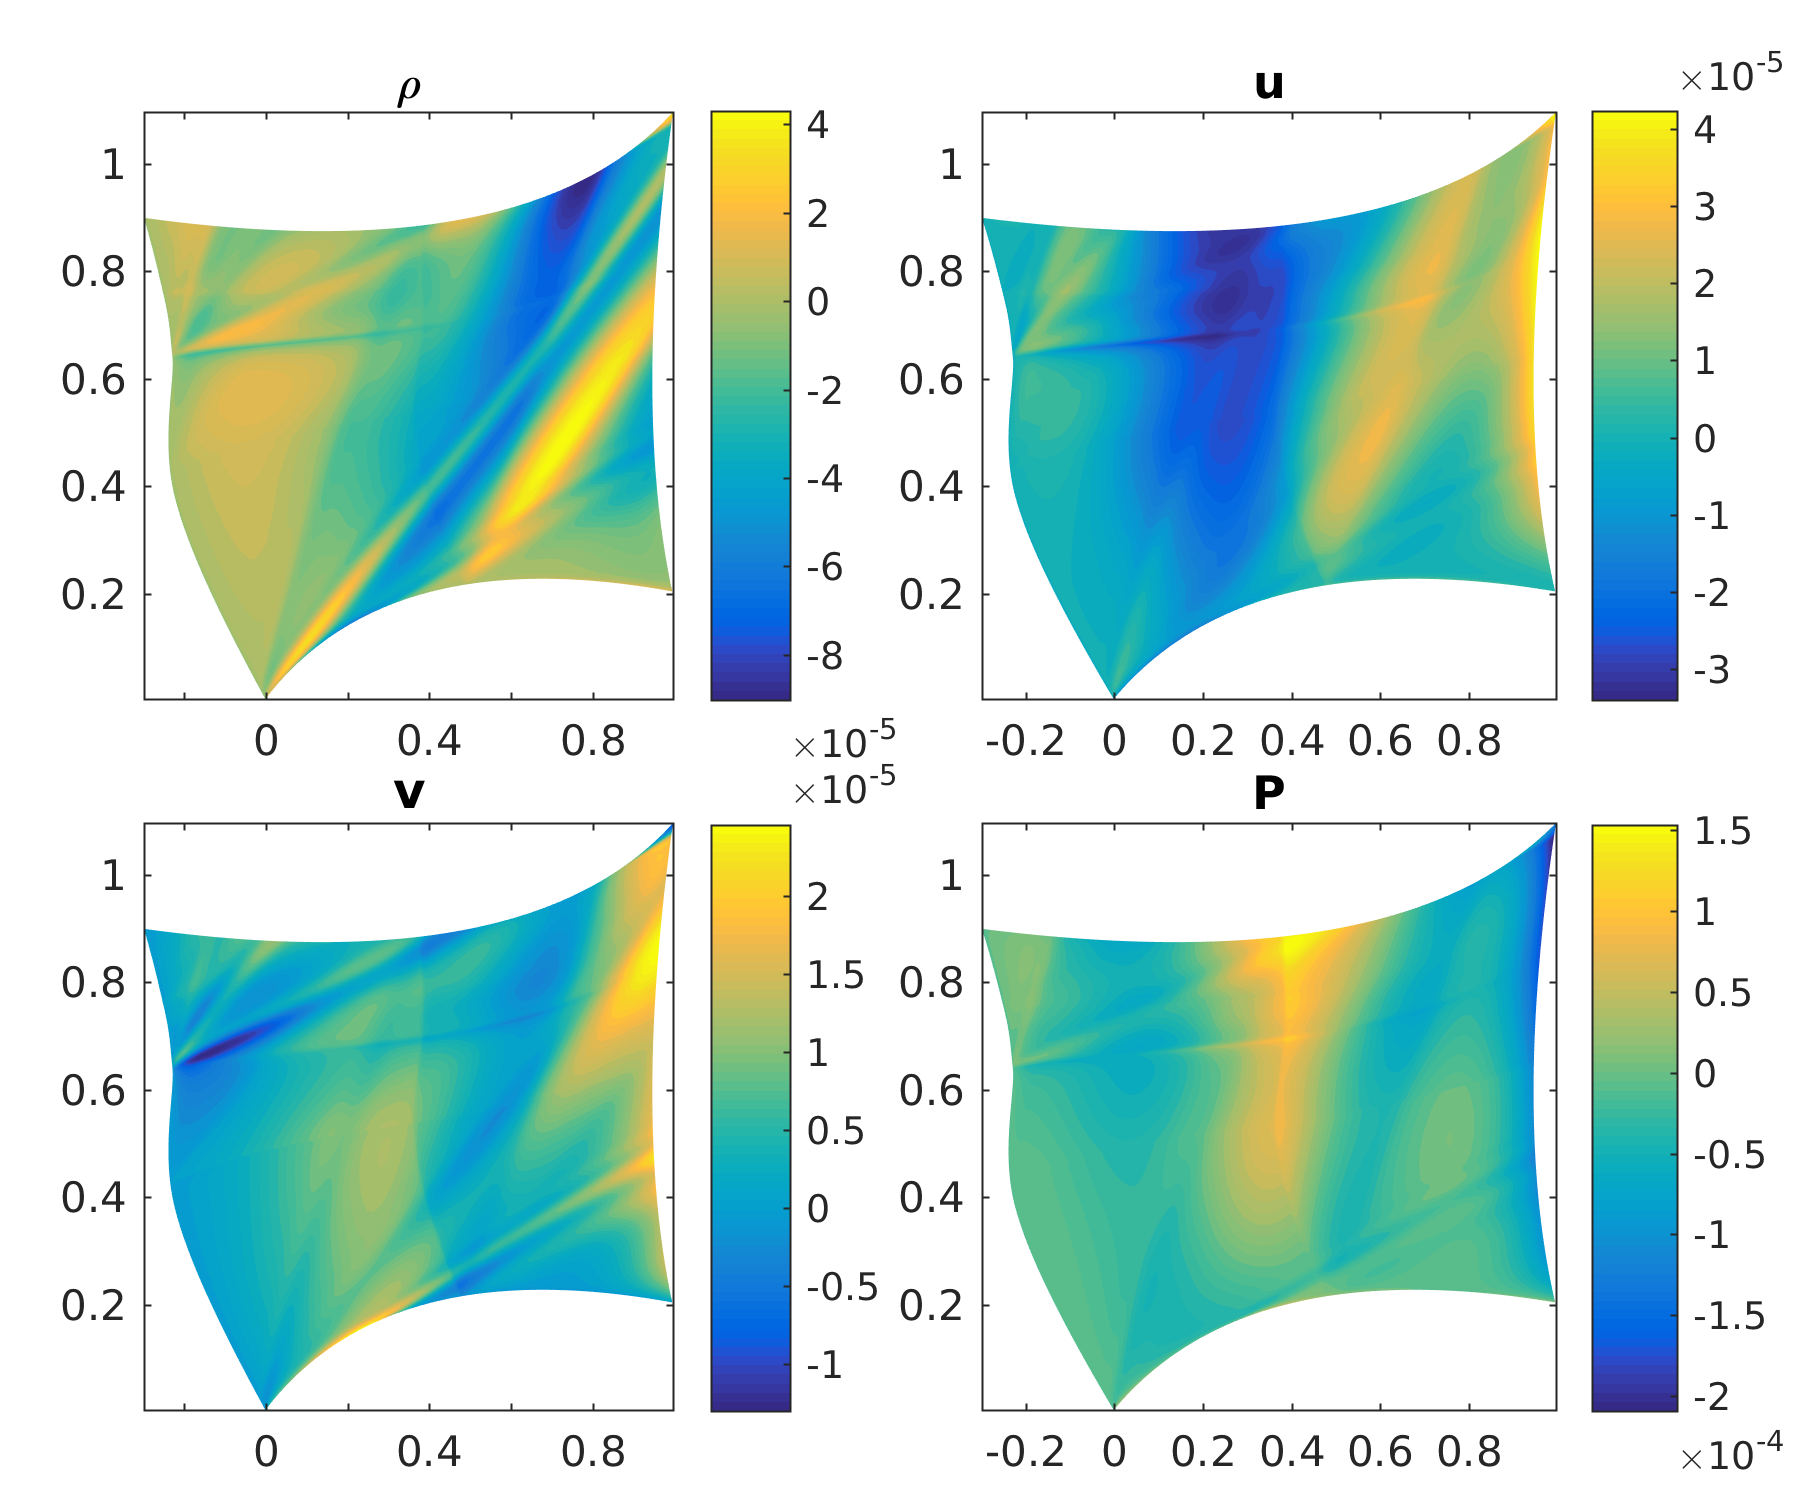
\includegraphics[width=\linewidth]{figures/MMS_mesh6_SS_DE}
  \caption{Local discretization error using 2nd order Van Leer FVS for the supersonic manufactured solution on the 257x257 mesh.}
  \label{fig:DESS}
  \endminipage\hfill
  \minipage{0.49\textwidth}
  \centering
  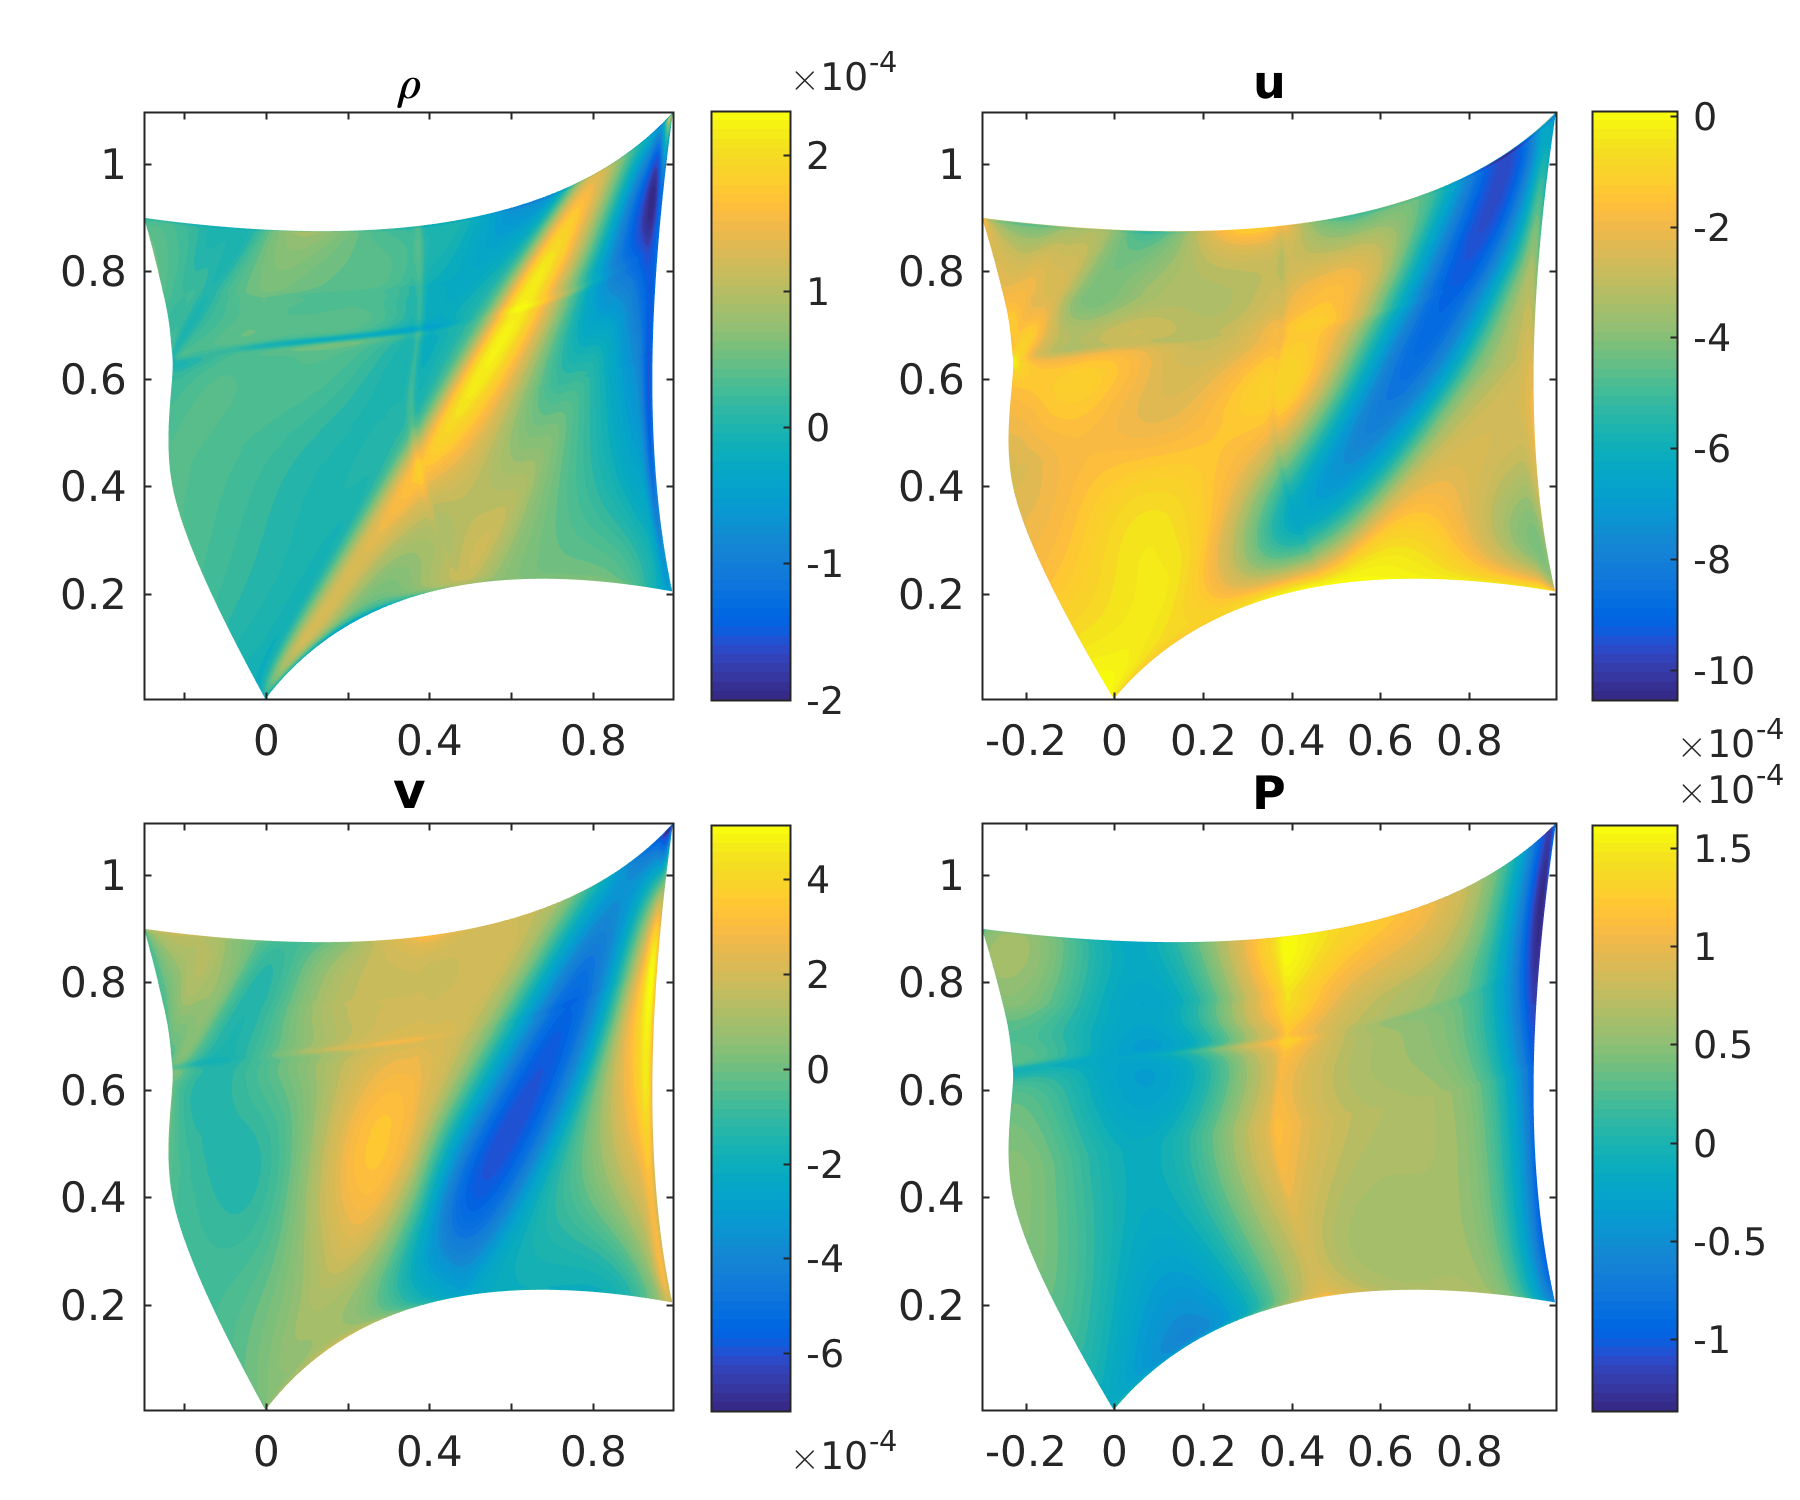
\includegraphics[width=\linewidth]{figures/MMS_mesh6_SB_DE}
  \caption{Local discretization error using 2nd order Van Leer FVS for the subsonic manufactured solution on the 257x257 mesh.}
\label{fig:DESB}
  \endminipage\hfill
\end{figure}

\subsection{Case 2: 30$^o$ Inlet}
Supersonic inflow through a 30$^o$ inlet was studied using the values in table~\ref{tbl:inlet} on a 417x129 mesh. Figure~\ref{fig:inletmesh} shows the mesh used for in the simulation. The boundary conditions consist of an inlet, outlet, lower slipwall, upper slipwall, and symmetric lower boundary. Figure~\ref{fig:inlet} show the solution on the finest grid to 1st order accuracy. The outlet pressure is determined through an integral average of the values along the outlet boundary, and was found to be $P_{o}\approx133.3\; Pa$. These can then be used to evaluate a total pressure which is related through the Mach number by 
\begin{equation}\label{eq:totalp}
  P_t = P\left[1+\frac{\gamma - 1}{2}M^2\right]^{\left(frac{\gamma}{\gamma - 1}\right)}
\end{equation}
where $\gamma = 1.4$. Using this the total pressure at the inlet is $1.86e6\;Pa$, and the numerical total pressure at the outlet is $5.017e5\;Pa$. Therefore the total pressure drop from inlet to outlet is $\Delta P_t=1.36e6\;Pa$

\begin{table}% no placement specified: defaults to here, top, bottom, page
  \begin{center}
    \caption{Inflow Conditions for the 30$^o$ inlet}
    \label{tbl:inlet}
    \begin{tabular}{rrr}
      Desc & Value & Unit \\\hline
      Mach &  4.0 & na \\
      Pressure &  12,270 & Pa \\
      Temperature & 217 & K
    \end{tabular}
  \end{center}
\end{table}

\begin{figure}[!htb]
  \centering
  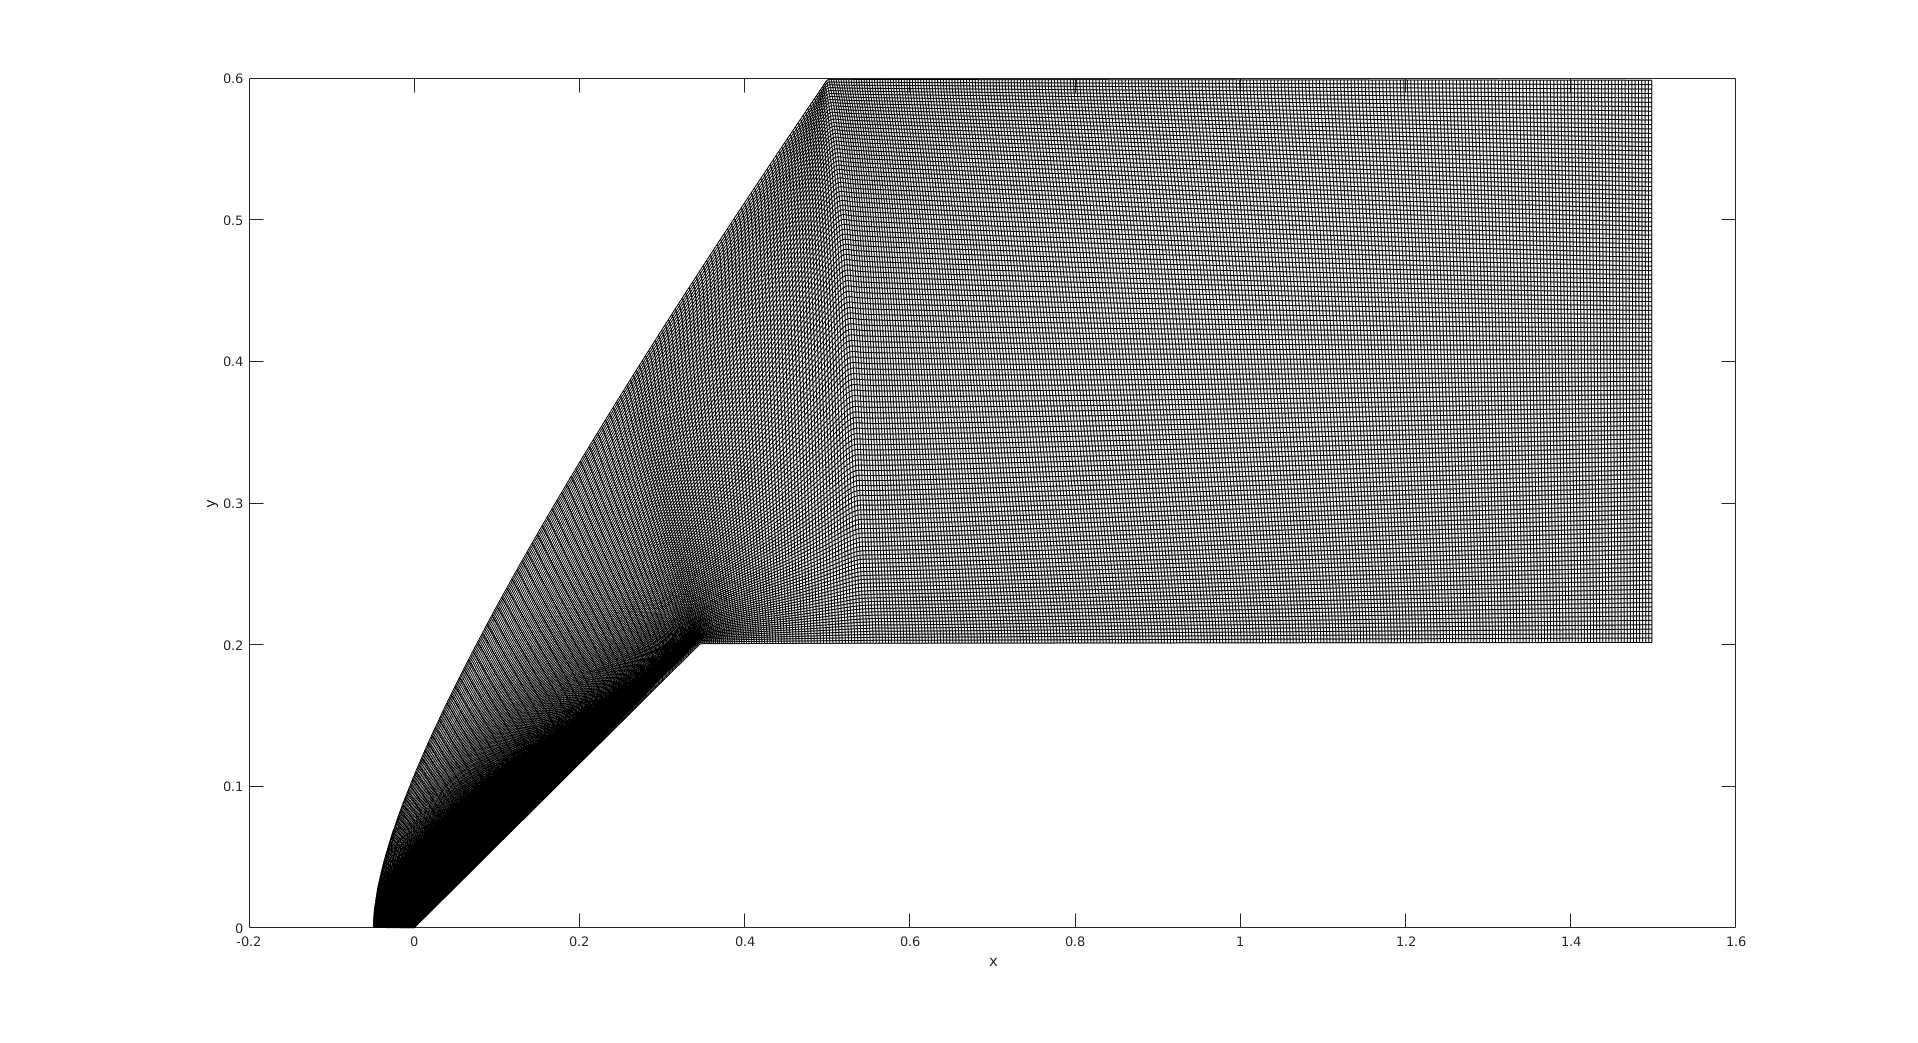
\includegraphics[width=0.5\linewidth]{figures/InletMesh4}
  \caption{ 30$^o$ inlet 417x129 mesh.}
  \label{fig:inletmesh}
\end{figure}

\begin{figure}[!htb]
  \centering
  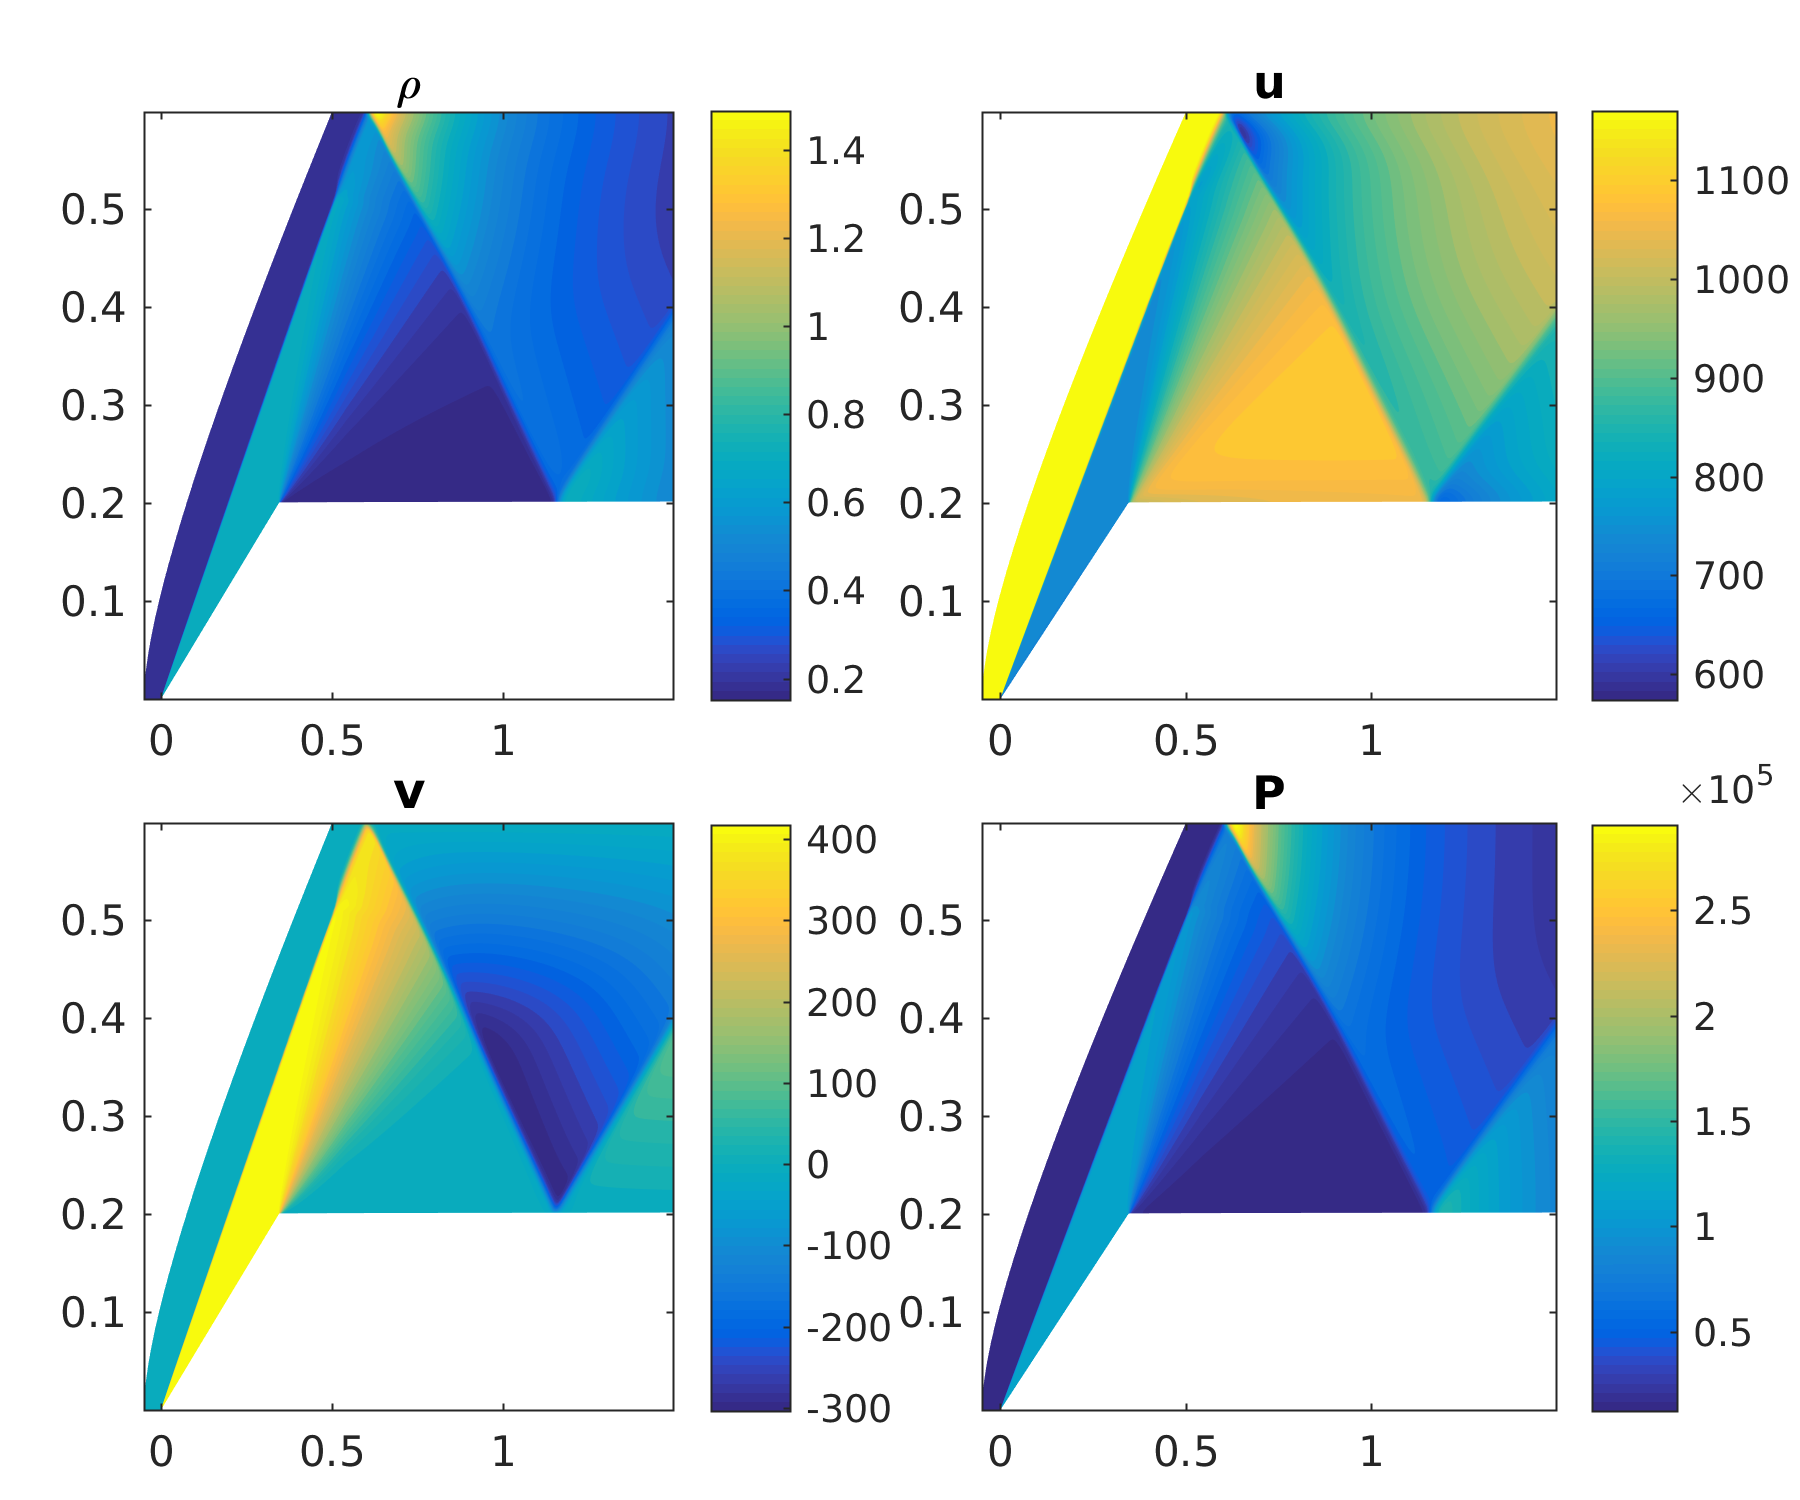
\includegraphics[width=0.75\linewidth]{figures/Inlet_mesh4_Soln}
  \caption{Numerical solution of the 30$^o$ inlet using 1st order Van Leer FVS on the 417x129 mesh.}
  \label{fig:inlet}
\end{figure}

\subsection{Case 3: NACA64A Airfoil}
Using $0^o$, and $8^o$, angle of attack (AOA) on a 385x105 size mesh estimation of the lift and drag were found. Initial conditions are described in table~\ref{tbl:0AOA} for $0^o$ AOA, and in table~\ref{tbl:8AOA} for $8^o$ AOA. The boundary conditions consists of farfield, periodic, and slipwall. The simulation used a mesh of 385x105, and is shown in figure~\ref{fig:nacamesh} which is used for both AOA's. The solutions for both AOA's are shown in figures~\ref{fig:naca0AO}, and~\ref{fig:naca8AO}. 

In figure~\ref{fig:naca0AO} the pressure$\cdot$area  can be used to find the force at the individual cells, this can then be integrated over to find an average force on the airfoil. This force can be related to the drag an lift which can be found experimentally. For $0^o$ AOA the drag and lift coefficients experimentally are $c_d = 0.00901$, and $c_l=0.009701$, respectively. These can then be used to get the drag per unit span, and the lift per unit span. The drag per unit span can be obtained by

\begin{equation}\label{eq:drag}
  D' = \frac{1}{2} c_d \rho_{\infty} V_{\infty}^2 c
\end{equation}
where $\rho_{\infty}$, and $V_{\infty}$, are found with the freestream conditions, and $c=0.1524m$ is the chord. The lift per unit span uses a nearly identical equation with the swap of $c_d$ to $c_l$. Evaluating this equation with the given free stream conditions results in a drag and lift per unit span of $D'=22.3321 \; N/m$, and $L'=24.0449\; N/m$. The numerically simulated values are $D'\approx = 20.6\; N/m$, and $L'\approx21.7\; N/m$, which are relatively in good agreement to the experimental values. Due to the symmetry of the airfoil the drag and lift coefficients are relatively close. If instead a NACA2415 airfoil was used the lift and drag would coefficients would differ more drastically.  

\begin{table}% no placement specified: defaults to here, top, bottom, page
  \begin{center}
    \caption{Freestream Conditions for the 0$^o$ AOA}
    \label{tbl:0AOA}
    \begin{tabular}{rrr}
      Desc & Value & Unit \\\hline
      Mach &  0.84 & na \\
      Pressure &  65,855.8 & Pa \\
      Temperature & 300 & K
    \end{tabular}
  \end{center}
\end{table}
\begin{table}% no placement specified: defaults to here, top, bottom, page
  \begin{center}
    \caption{Freestream Conditions for the 8$^o$ AOA}
    \label{tbl:8AOA}
    \begin{tabular}{rrr}
      Description & Value & Unit \\\hline
      Mach &  0.75 & na \\
      Pressure &  67,243.5 & Pa \\
      Temperature & 300 & K
    \end{tabular}
  \end{center}
\end{table}


\begin{figure}[!htb]
  \centering
  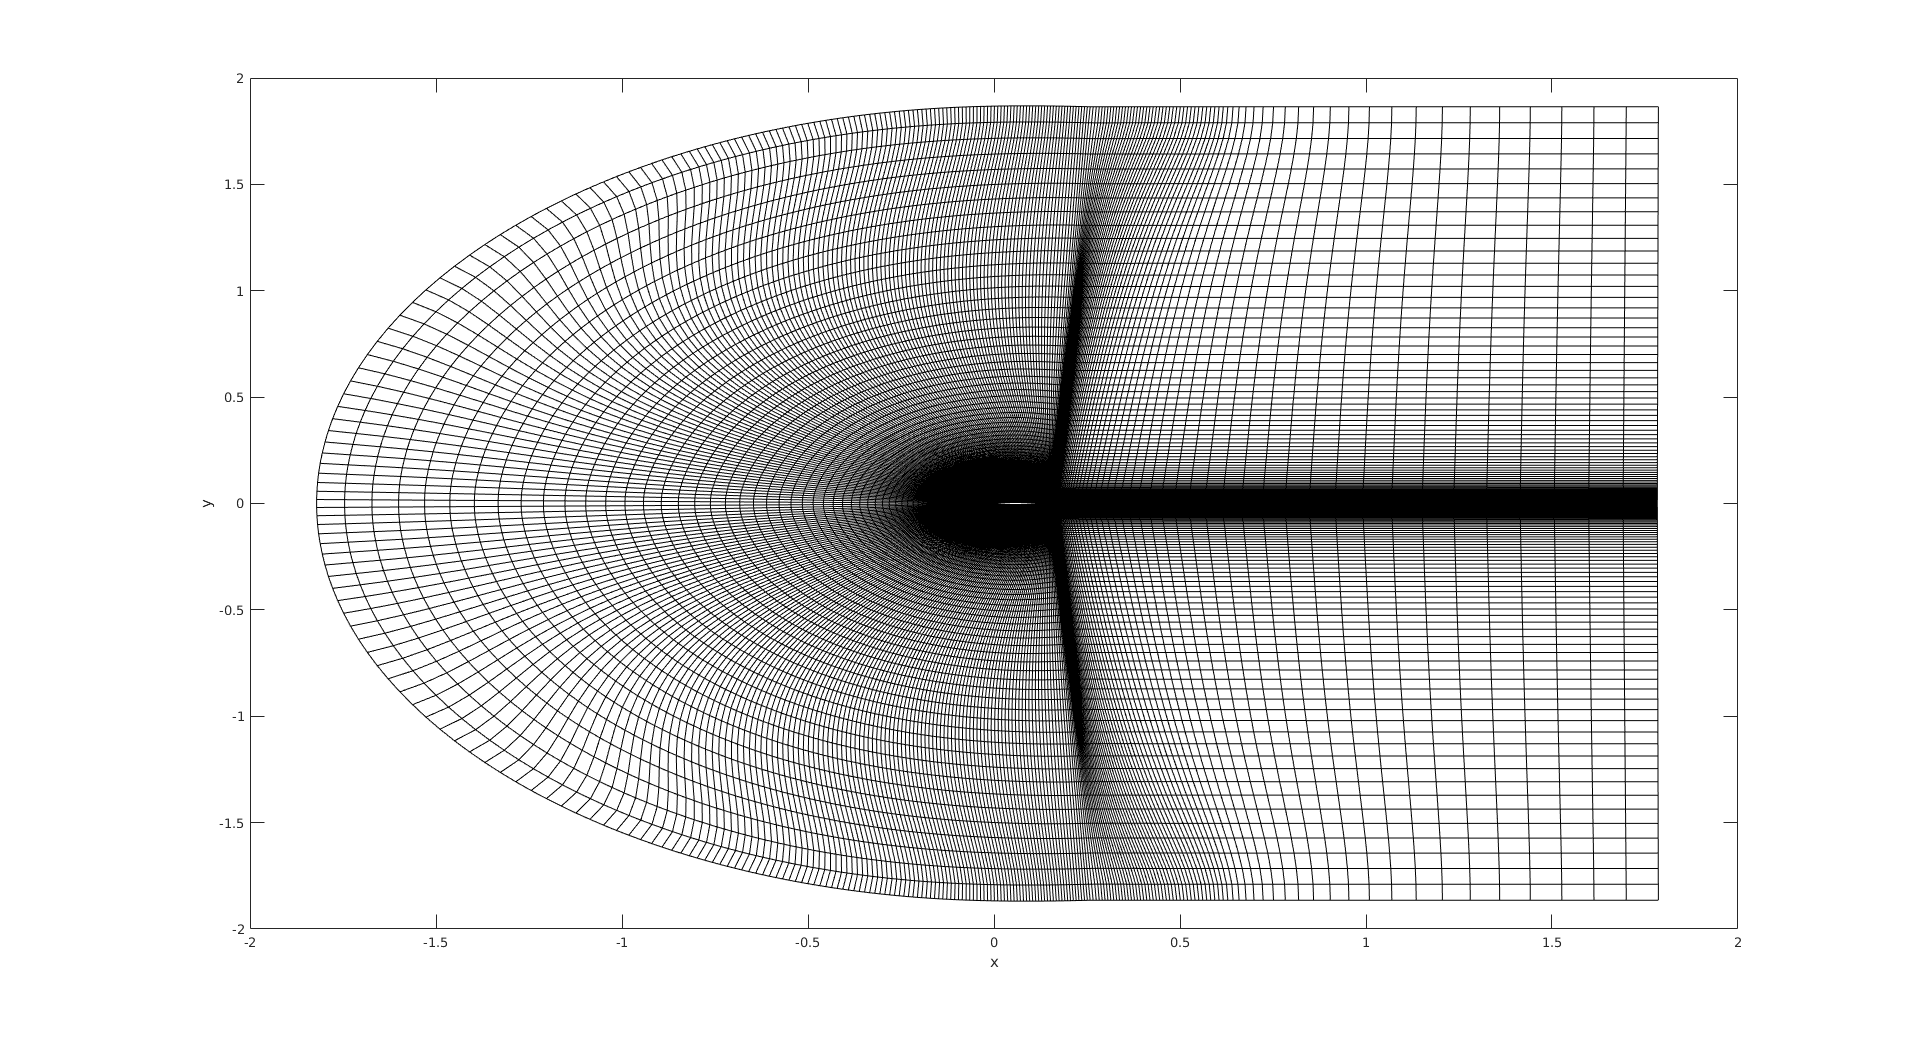
\includegraphics[width=0.5\linewidth]{figures/NACAMesh4}
  \caption{ NACA64A airfoil 385x105 mesh.}
  \label{fig:nacamesh}
\end{figure}

\begin{figure}[!htb]
  \centering
  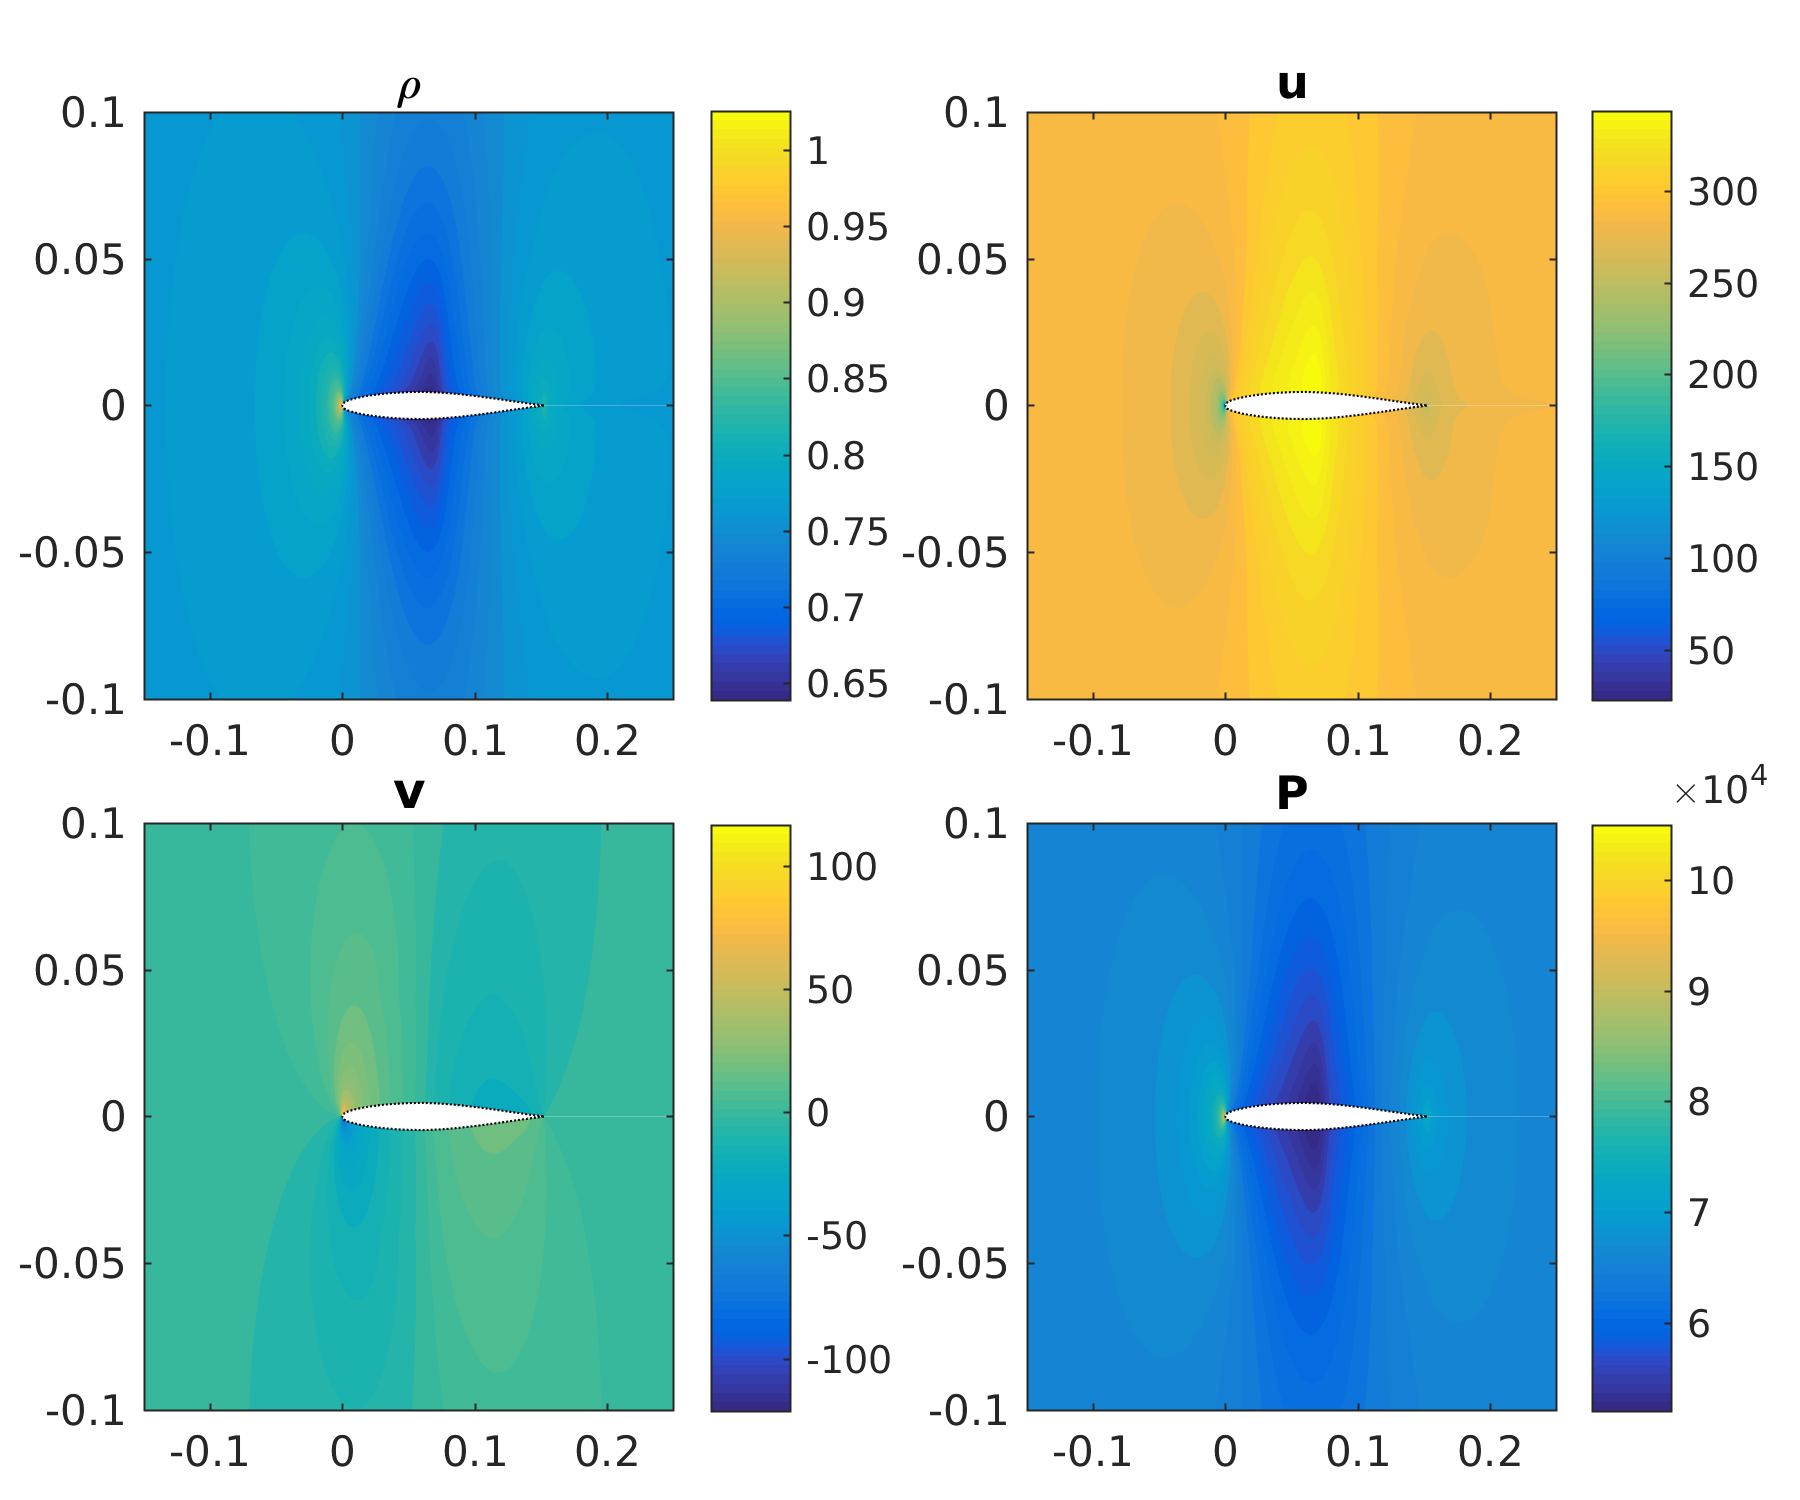
\includegraphics[width=0.75\linewidth]{figures/NACA_mesh4_A0_Soln}
  \caption{Cropped numerical solution of NACA airfoil with $8^o$ AOA using 1st order Roe FDS on a 417x129 mesh.}
  \label{fig:naca0AO}
\end{figure}

\begin{figure}[!htb]
  \centering
  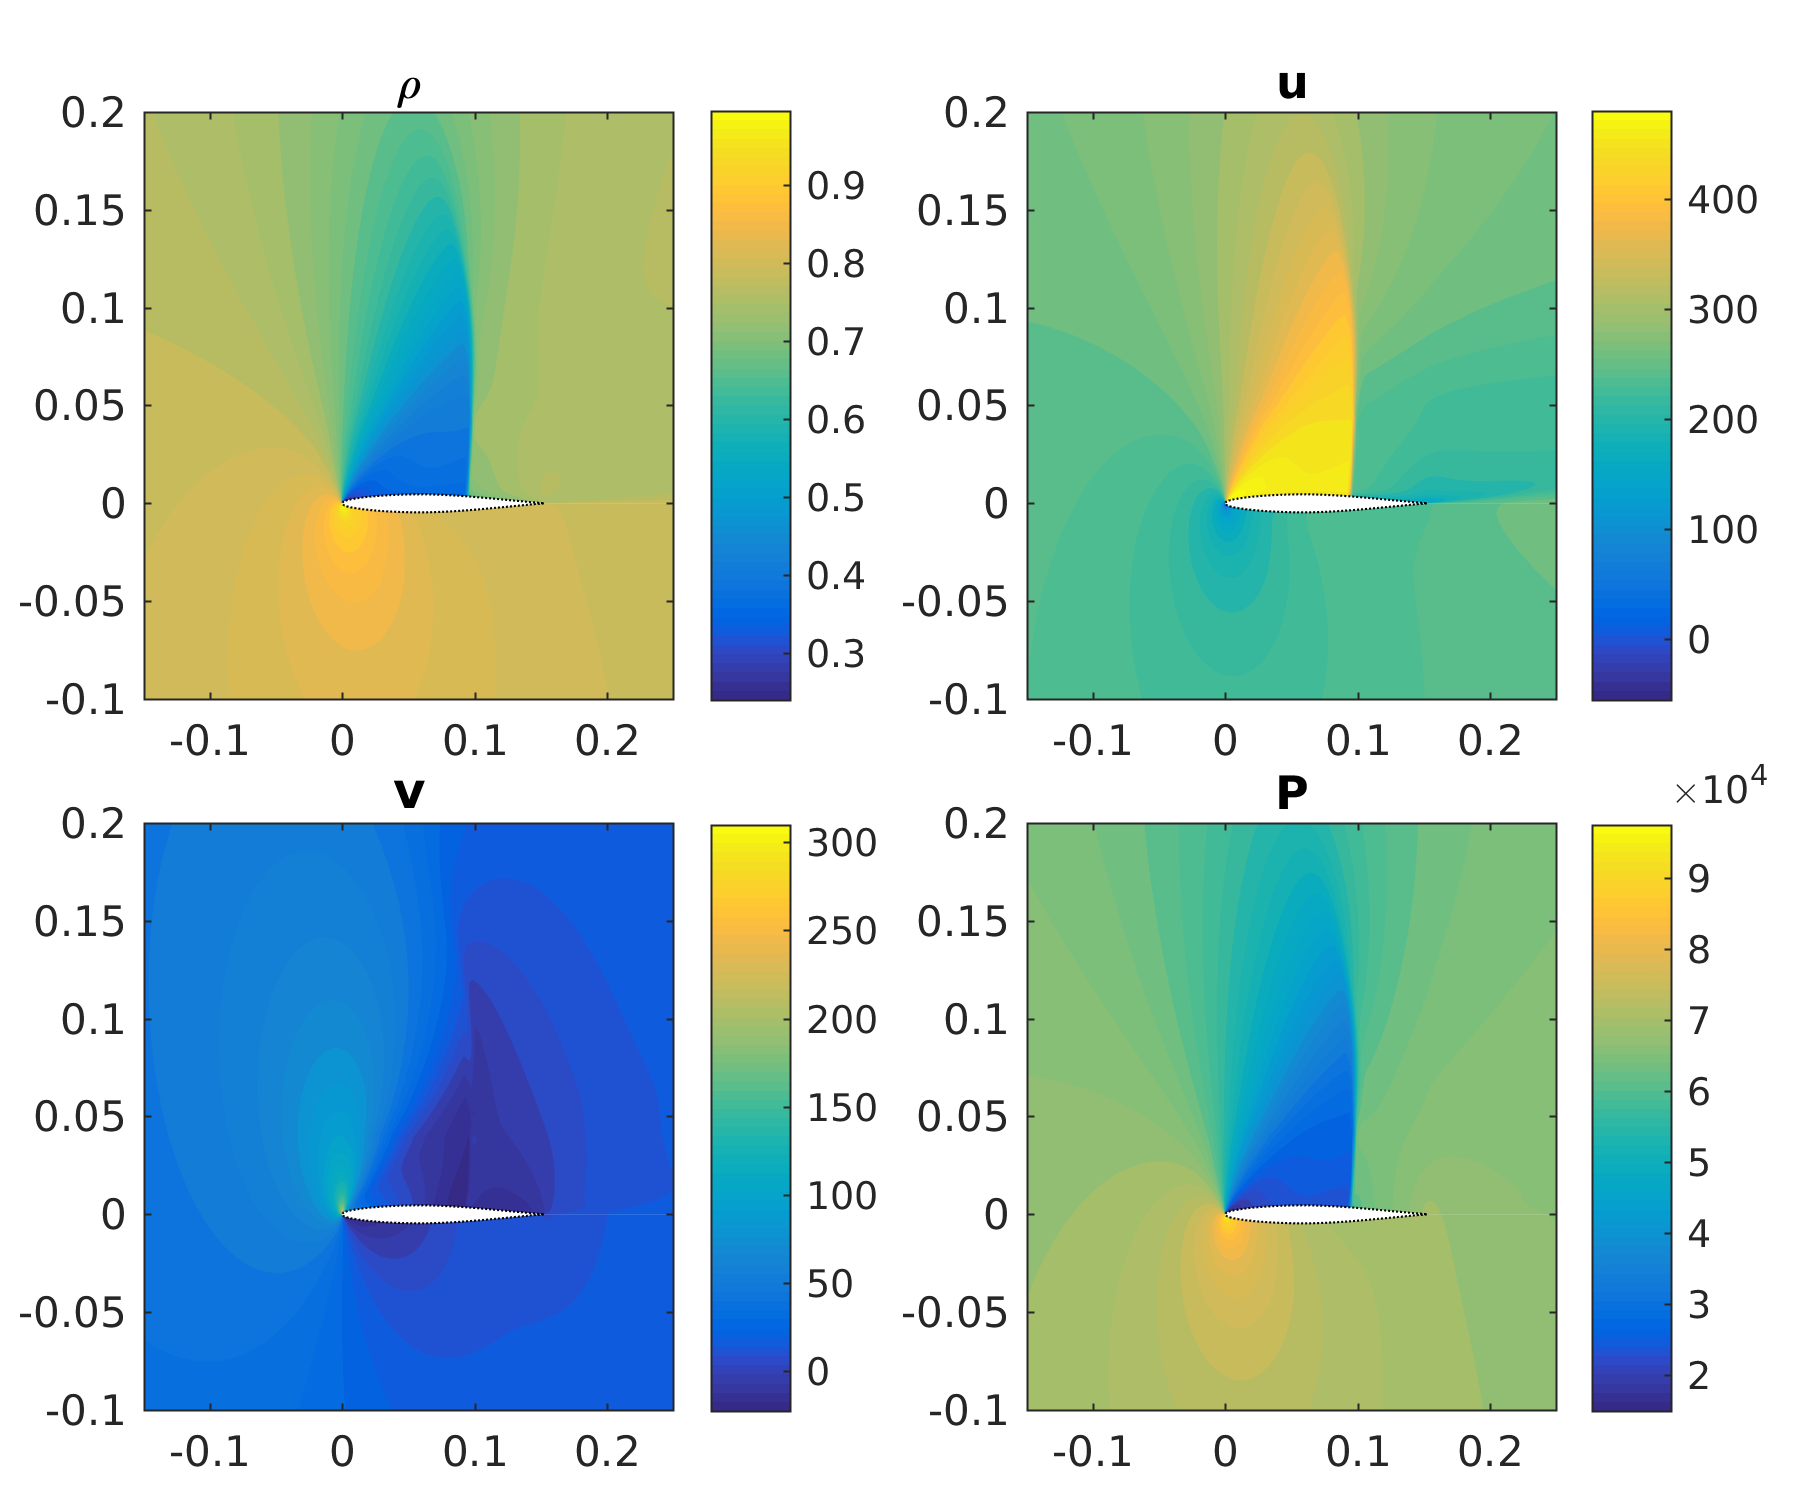
\includegraphics[width=0.75\linewidth]{figures/NACA_mesh4_A8_Soln}
  \caption{Cropped numerical solution of NACA airfoil with $8^o$ AOA using 1st order Roe FDS on a 417x129 mesh.}
  \label{fig:naca8AO}
\end{figure}

\section{Conclusion}

A FVM scheme was validated using MMS, and benchmarked with a supersonic 30$^o$ inlet, and flow around an NACA64A airfoil. MUSCL extrapolation was used to get reconstructed conserved variables at the interfaces. Numerical flux was determined by Van Leer's FVS, and Roe's FDS. An average total pressure loss was determined for the 30$^o$ inlet. The drag, and lift, per unit span were compared to experimental results, and showed good agreement with 0$^o$ AOA. 

\pagebreak
\bibliographystyle{plainnat}
\bibliography{reference}
\end{document}
